\documentclass[journal]{IEEEtran}
\usepackage{graphicx}
\usepackage{amsmath}
\usepackage{amssymb}
\usepackage{amsxtra}
\usepackage{amstext}
\usepackage{latexsym}
\usepackage{dsfont}
\usepackage{float}
\usepackage{cite}
\usepackage{subcaption}
\usepackage{multirow}
\ifCLASSINFOpdf
%\usepackage[pdftex]{graphicx}
  % declare the path(s) where your graphic files are
  % \graphicspath{{../pdf/}{../jpeg/}}
  % and their extensions so you won't have to specify these with
  % every instance of \includegraphics
  % \DeclareGraphicsExtensions{.pdf,.jpeg,.png}
\else

\fi

\hyphenation{op-tical net-works semi-conduc-tor}


\begin{document}
\title{Performance analysis of linear polarization antenna in 2.45 GHz on-body communications}

\author{Lingfeng~Liu,~\IEEEmembership{}
        Xiaonan~Wang,~\IEEEmembership{}
        and~Peng~Zhang.~\IEEEmembership{}% <-this % stops a space
\thanks{Lingfeng liu, Xiaonan Wang and Zhang Peng are with the Signal Information Engineering school, East China
Jiaotong University, China, e-mail: lingf.liu@gmail.com.}% <-this % stops a space
\thanks{This work is supported by the Natural Science Foundation of China (NSFC) under grant No. 81460275.}% <-this %
stops a space
\thanks{Manuscript submitted July 4, 2017.}}


\maketitle

\begin{abstract}
On-body channels show highly polarization selectivity with respect to the orientation of the transmit and receiving
antennas, while the body coupling and scattering effects in reverse affect the antenna polarization characteristics
in near-field. In this paper, three kinds of compact linearly polarized antennas, the inverted-F antenna, the MIFA
antenna, and the printed dipole antenna, are designed and are analyzed for their polarization performance above the
body trunk via numerical simulations. A simplified three-layered human chest model including skin, fat, and muscle
tissues is applied. The return loss, bandwidth, and the radiation pattern of the investigated antennas are
found to be affected by the relative orientation and distance between the antennas and the trunk, indicating the
necessity of the antenna placement optimization for realistic on-body communication devices.
\end{abstract}

% Note that keywords are not normally used for peerreview papers.
\begin{IEEEkeywords}
IFA, MIFA, printed dipole, horizontal polarization, vertical polarization, Body Area Network(BAN).
\end{IEEEkeywords}

\IEEEpeerreviewmaketitle



\section{Introduction}
\IEEEPARstart{R}{cent} years, wireless body area networks (WBANs) have drawn great interest for design and optimization
of ulta-low powered wearable communication devices in health care and medical applications. Due to the complexity of the body, propagation along and around the body show distinct decaying and variation patterns. The complex body coupling and scattering effects  bring challenges in the design of miniature on-body antennas. Several papers have been written to show the reliance of antenna radiation efficiency, its return loss and resonant frequency and its radiation pattern on the dielectric properties of human tissues \cite{1, 2}. Characteristics of antennas and on-body channels have been widely studied \cite{3}-\cite{6}. For realistic wearable on-body communications in the other aspects, the antennas are often mounted on the torso or limbs to obtain optimal performance, as shown by study in \cite{7}. Studies as \cite{8, 9} also reveal the possibility to explore the polarization spatial diversity in on-body channels to improve the performance of e.g. relaying and Multi-Input Multi-Output (MIMO) in WBANs.

On-body channels show great spatial with respect to the placements of the antennas and polarization selectivity with respect to the orientation of the antennas both on static and dynamic bodies \cite{10, 11}. Recent researches in the design of on-body matched antennas cover several factors like size reduction, bending capability, bandwidth requirement, SAR evaluation, biocompatibility, radiation and coupling effects \cite{12}. It calls for on-body antenna optimization in order to gain the channel polarization gain or polarization diversity, to further lower the power consumption, or to reduce the link loss \cite{13}. For optimization design of multi-polarization antennas, we should consider how to design the antenna to ensure every polarization component can achieve better channel, and to investigate the antenna's radiation gain. Before analyzing any complex polarization antennas, we must understand the basic polarization performance via linearly polarized antennas, therefore, we choose linearly polarized antennas and study the antennas placed on the surface of the torso.

There are several numbers of researches on open literature which present the antenna performance close to the human body, e.g., \cite{14}-\cite{16}. The design of on-body antennas usually undergoes two problems. First, while most of the on-body antennas are integrated in the garment or attached to the skin \cite{17, 18}, the human body may exert complex electromagnetic impact to the antenna's performance \cite{19, 20}. Second, even the human body has been included during the design of the on-body antennas, the placement variation of the antennas can deeply affect the actual polarization performance of the on-body antennas. including the distance and orientation of the antennas to the skin, and the part of the body, arms, chest, etc., the antennas located. Therefore, we study the impact of antenna orientation and placement on the antenna when the antenna placed in other locations may not be appropriate, or the body's movement will affect the performance of the antenna.

To study the impacts of these factors to the on-body antenna polarization performance, in this work, we introduce three compact types of linearly polarized antennas designed at 2.4 GHz placed on the surface of the torso. A simplified three-layered human chest model is applied. The antenna performance include return loss, bandwidth and radiation pattern are investigated and compared at various antenna-skin distances and at different orientation of the antennas relative to the skin.

This paper is divided into five parts. Section \ref{sec:antenna_design} introduces the design and optimization of the
linearly polarized antennas. Section \ref{sec:body_model} presents the layered human chest model. Section \ref{sec:analysis} analyzes the polarization performance of the antennas. And finally, summaries are concluded in section \ref{sec:conclusion}.

\section{Antenna design}
There are three types of linearly polarized microstrip antennas designed and investigated in the study, which are the
IFA, MIFA and printed dipole antennas. The selected antennas are in compact shape, simple structure, low production
costs, and relatively easy to get matched. The structures \cite{21} and initial geometry values of the antennas are summarized in Fig. \ref{fig:1} and Tab. \ref{tab:1}. All the antennas are fabricated on PCB and operates in the 2.4 GHz ISM band with center frequency of 2.45 GHz. The dielectric layer is made of FR4 with $\epsilon_{r}$=4.4 \cite{22}. The antenna is
simulated by Ansoft HFSS 13.0$^{\textcircled{R}}$. The antennas are firstly optimized in free space by tuning their resonant frequency to 2.45 GHz. The structure and performance of the optimized antennas are summarized in Fig. \ref{fig:2} and table \ref{tab:ant_optimized}.

\begin{figure}[!htb]
\centering
\begin{subfigure}[b]{0.24\textwidth}

\includegraphics[width=\textwidth]{figs/1a.eps}
\caption{IFA}
\label{fig:a}	
\end{subfigure}		
\begin{subfigure}[b]{0.24\textwidth}
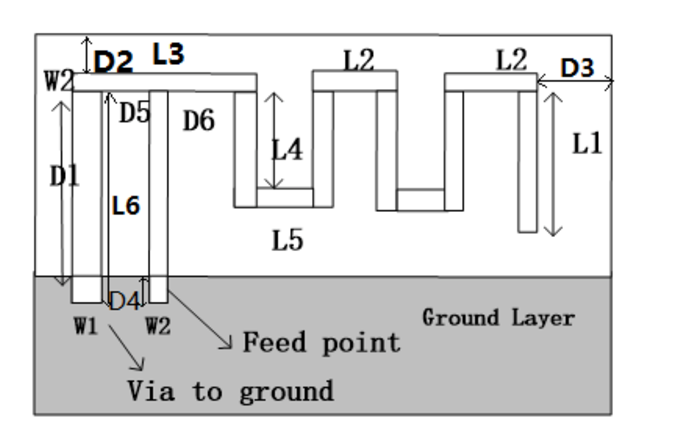
\includegraphics[width=\textwidth]{figs/1b.eps}
\caption{MIFA}
\label{fig:b}
\end{subfigure}
\begin{subfigure}[b]{0.24\textwidth}
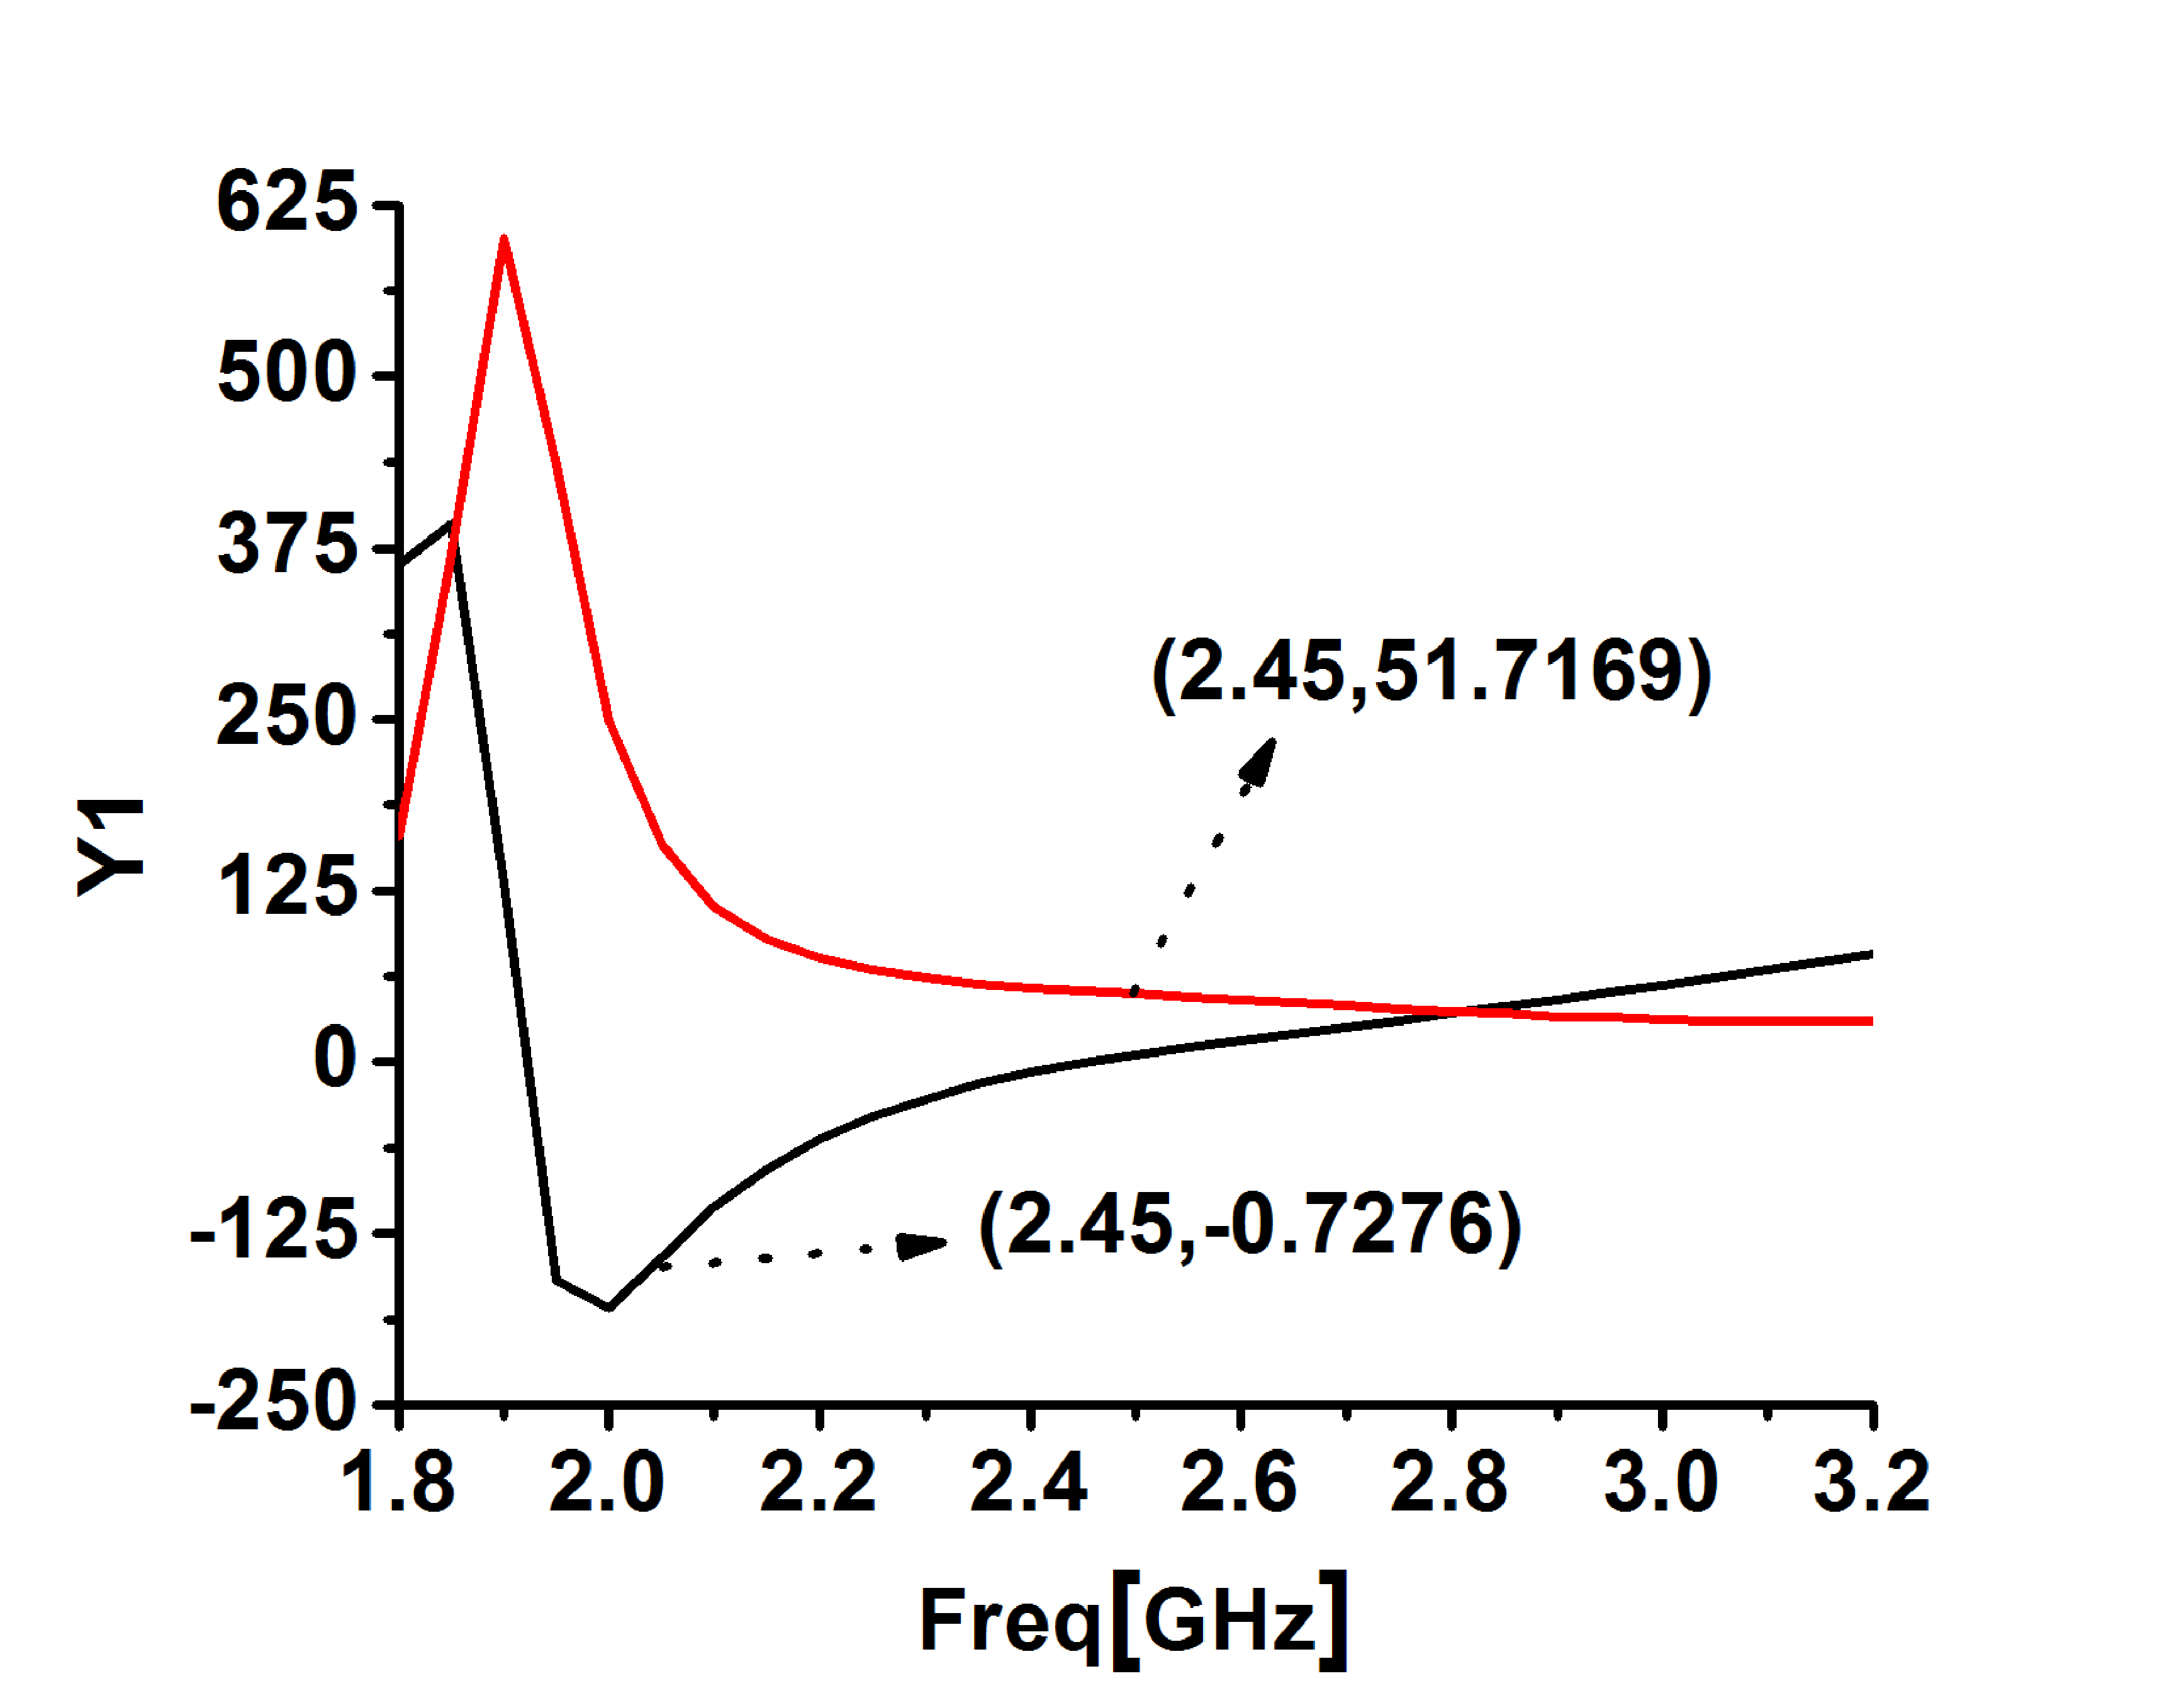
\includegraphics[width=\textwidth]{figs/1c.eps}
\caption{Dipole}
\label{fig:c}
\end{subfigure}
\caption{Parameters of  three antennas}
\label{fig:1}
\end{figure}

\begin{table}[!ht]
\centering
\begin{tabular}{|c|c|c|}
\hline
Antennas&Variable&Initial Values(mm)\\
\hline
\multirow{7}{*}{IFA}&L&16.2\\
&H&3.8\\
&S&5\\
&W&1\\
&SubH&0.8\\
&GndX&50\\
&GndY&90\\
\hline
\multirow{8}{*}{Dipole}&H&11.6\\
&W1&3\\
&L1&22\\
&W2&3\\
&L2&21\\
&L3&10\\
&L4&12\\
&W3&3\\
\hline
\multirow{8}{*}{MIFA}&D1&0.5\\
&D2&0.3\\
&D3&0.3\\
&D4&0.5\\
&D5&1.4\\
&D6&1.7\\
&L1&3.3\\
&L2&2.7\\
&L3&5\\
&L4&2.64\\
&L5&2\\
&L6&4.9\\
&W1&0.9\\
&W2&0.5\\
\hline
\end{tabular}
\caption{Variable definition}
\label{tab:1}
\end{table}

\begin{figure}[!htb]
\centering
\begin{subfigure}[b]{0.24\textwidth}
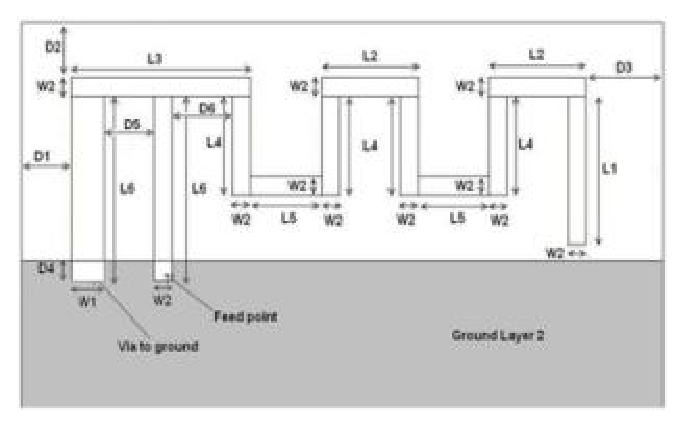
\includegraphics[width=\textwidth]{figs/2a.eps}
\caption{IFA}
\label{fig:2a}	
\end{subfigure}		
\begin{subfigure}[b]{0.24\textwidth}
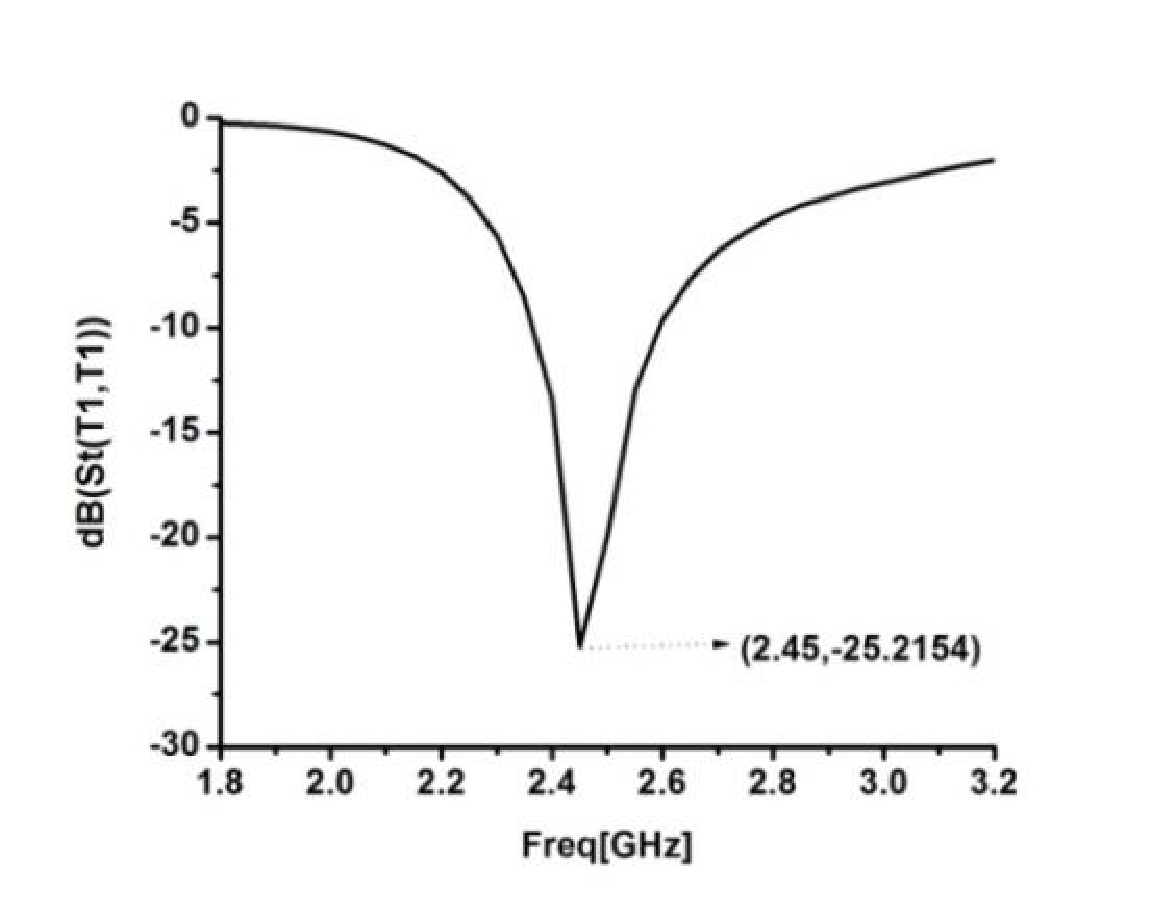
\includegraphics[width=\textwidth]{figs/2b.eps}
\caption{MIFA}
\label{fig:2b}
\end{subfigure}
\begin{subfigure}[b]{0.24\textwidth}
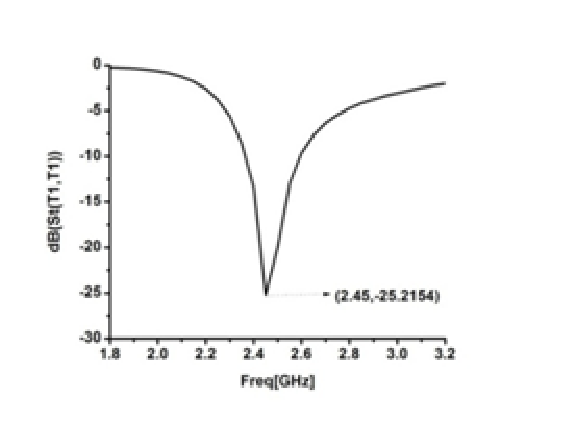
\includegraphics[width=\textwidth]{figs/2c.eps}
\caption{Dipole}
\label{fig:2c}
\end{subfigure}
\caption{Optimized $S_{11}$}
\label{fig:2}
\end{figure}

\section{Human body modeling}
The major difficulty of modeling the human body is that the body is composed of various biological tissues in different
shapes and electromagnetic properties. Most of the biological tissues are non-uniform dispersion medium and hence
can't be accurately described as a uniform model. To alleviate the complexity of human body modeling, it is suggested
to model different parts of the body respectively. Moreover, as the antenna performance in realistic environments is
simultaneously subjected to the body shape and environment, we choose simulation to isolate the environment
interference in the analysis.

\begin{figure}[!htb]
\centering
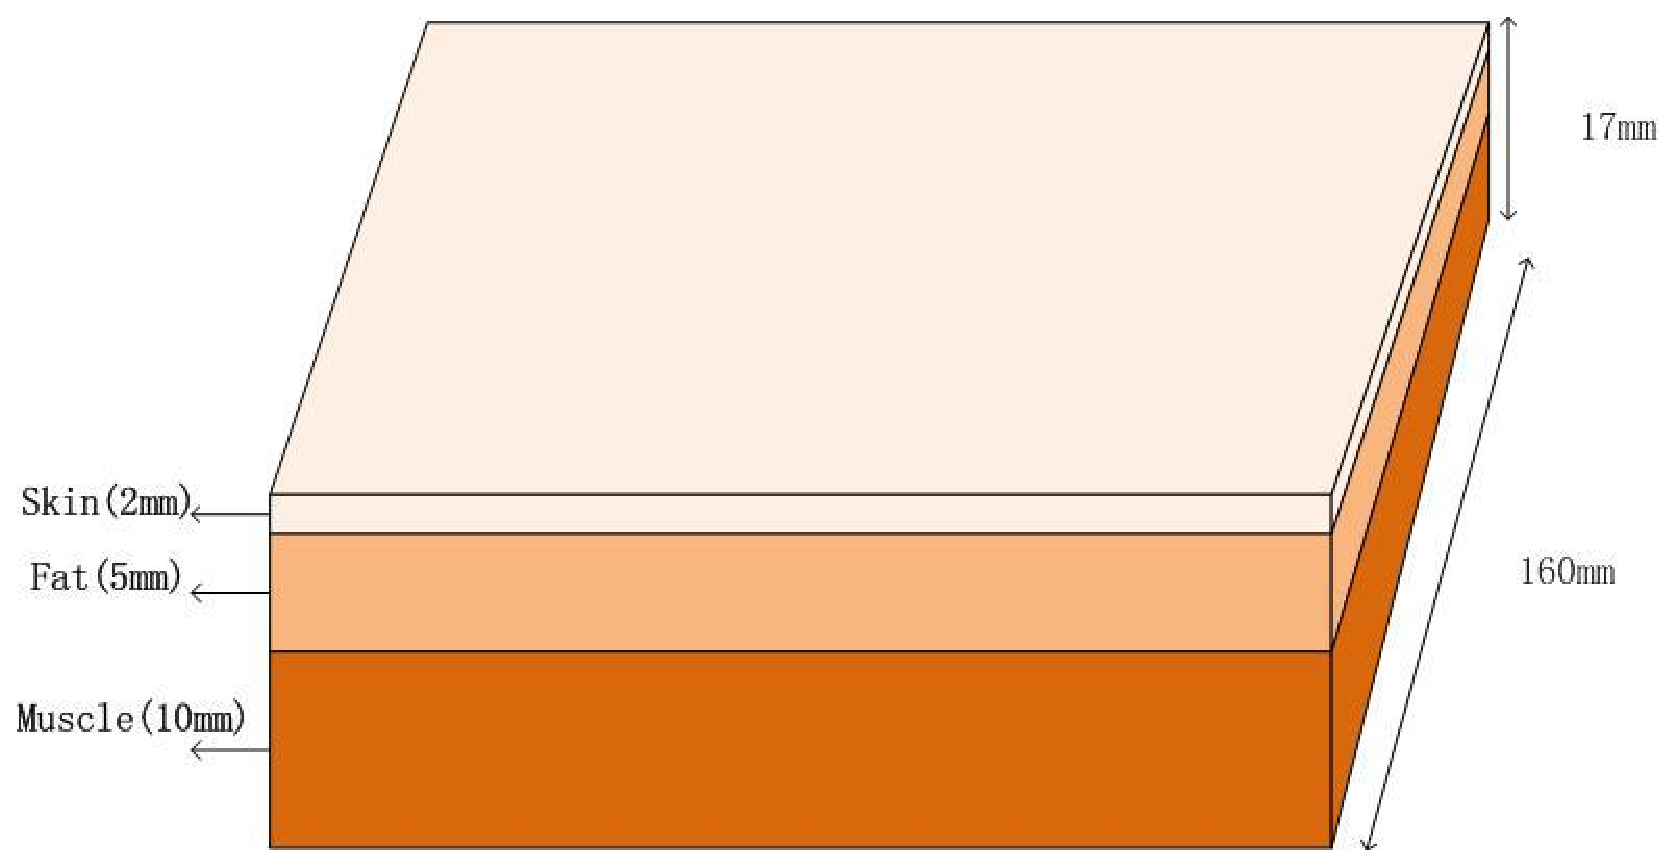
\includegraphics[width=0.4\textwidth]{figs/4.eps}
\caption{Layer chest modeling}
\label{fig:4}	
\end{figure}

\begin{figure}[!htb]
\centering
\begin{subfigure}[b]{0.24\textwidth}
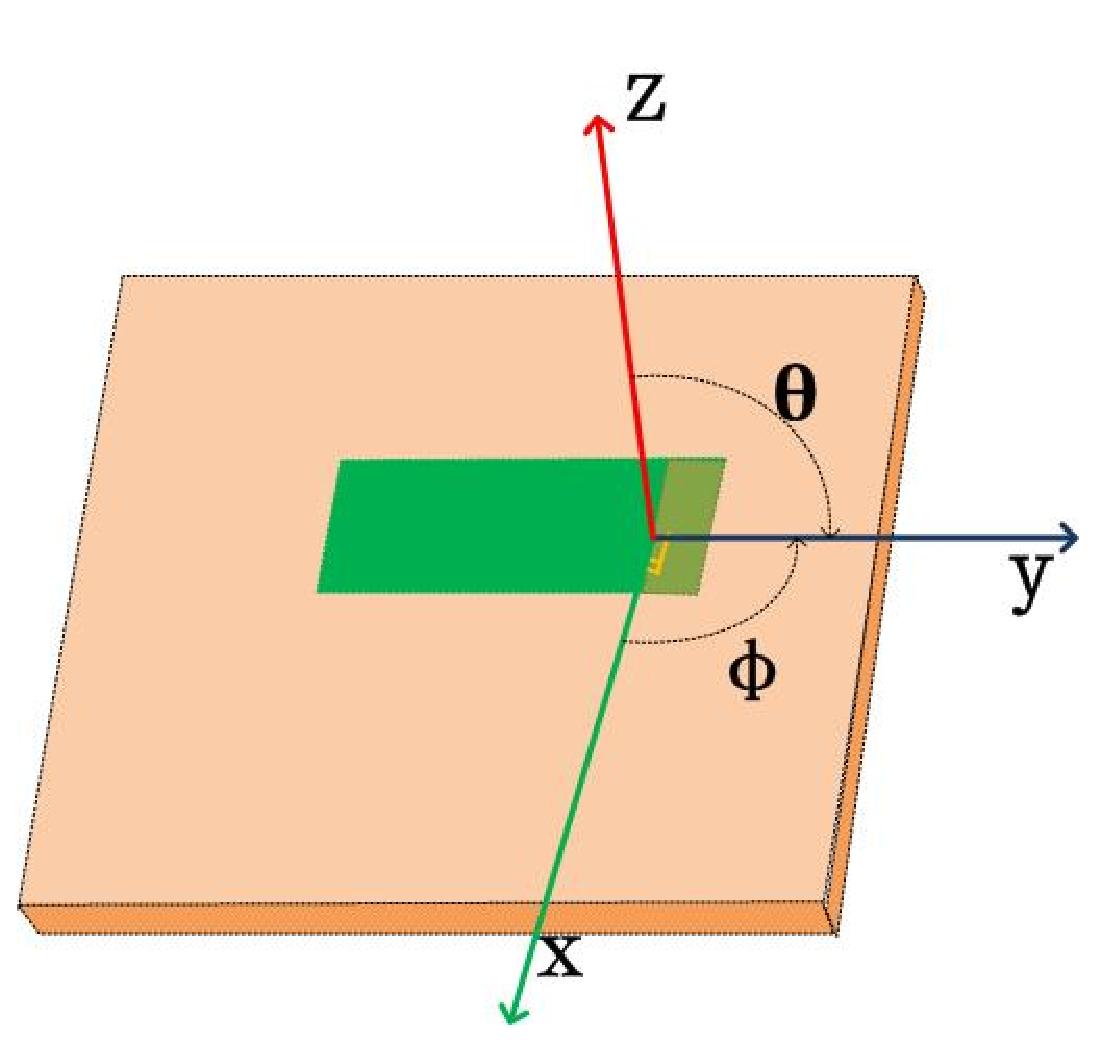
\includegraphics[width=\textwidth]{figs/3a.eps}
\caption{Horizontal polarization}
\label{fig:3a}	
\end{subfigure}		
\begin{subfigure}[b]{0.24\textwidth}
\includegraphics[width=\textwidth]{figs/3b.eps}
\caption{Vertical polarization}
\label{fig:3b}
\end{subfigure}
\begin{subfigure}[b]{0.24\textwidth}
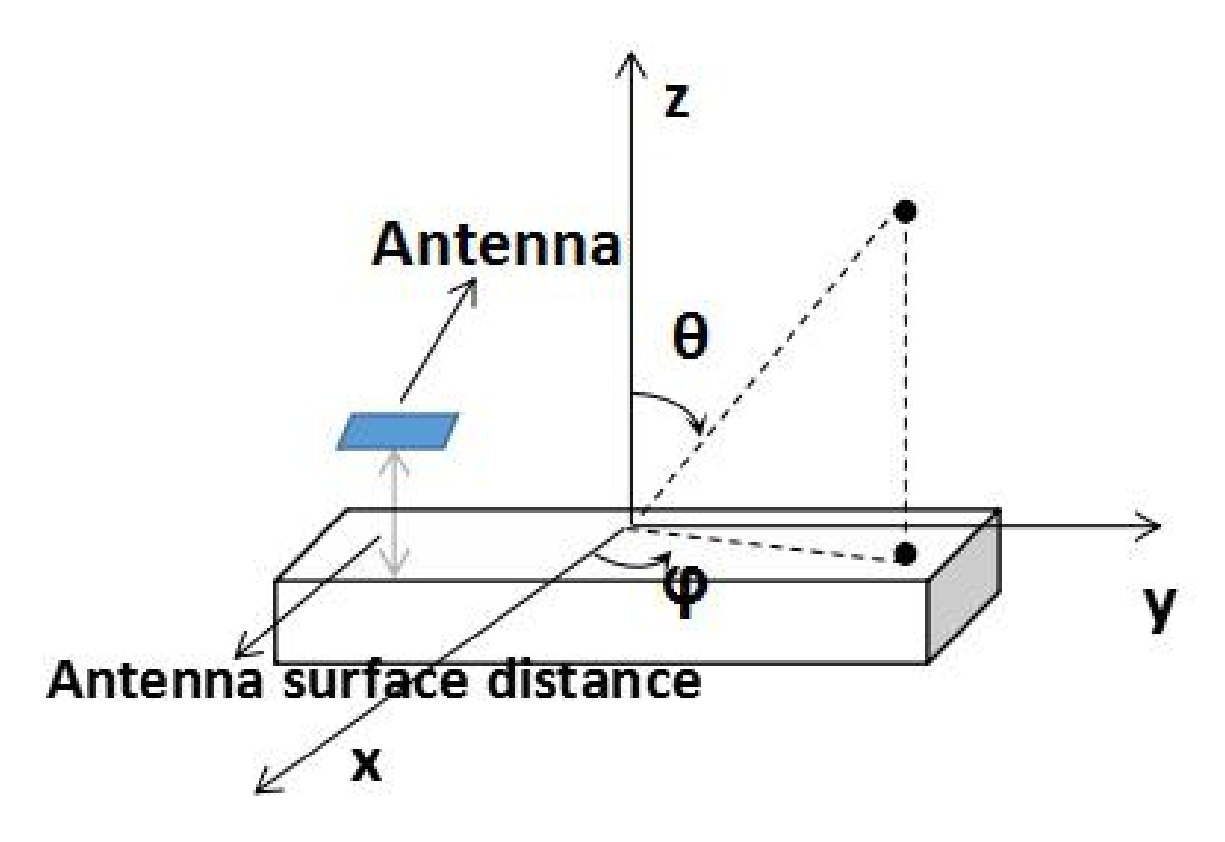
\includegraphics[width=\textwidth]{figs/3c.eps}
\caption{Definition of antenna and body surface distance}
\label{fig:3c}
\end{subfigure}
\caption{Polarization and geometry definition}
\label{fig:3}
\end{figure}

We focus on the chest part of the torso, whose structure can be approximated as a cuboid composed of three-layered
biological tissues as suggested in \cite{23}. As shown in Fig. \ref{fig:4}, the three-layer structure of the skin layer
(2 mm), fat layer (5 mm) and muscle layer (10 mm) was set from top to the bottom, and the dimension of the cuboid is
200 mm by 160 mm by 17 mm. Considering that the 2.4 GHz signal is rapidly attenuated in human body, this structure is
considered to be able to adequately simulate the chest. Dielectric constant and other electrical characteristics
\cite{24} are derived from human body and are shown in Tab. \ref{tab:2}.

On-body antennas are usually not directly attached to the skin, therefore we place the antenna at certain distance from
the body as shown in Fig. \ref{fig:3c}. $\theta$ and $\varphi$ are the angles between the Z axis and the Y axis, the X axis and the Y axis, respectively. When the antenna ground plate is parallel to the human body model as shown in Fig. \ref{fig:3a}, we call it horizontal polarization, and when the antenna ground is placed vertically with the surface of the human body as shown in Fig. \ref{fig:3b}, we call it vertical polarization. We define the XZ plane as the E-plane, and the XY plane is defined as the H-plane.

\begin{table}[!htb]
\centering
\begin{tabular}{|c|c|c|}
\hline
Tissue&$\epsilon_{r}$&$\sigma$\\
\hline
Skin&38.0066&1.4638\\
\hline
Muscle&52.7295&1.7388\\
Fat&10.8206&0.2680\\
\hline
\end{tabular}
\caption{Chest model parameters at 2.45 GHZ}
\label{tab:2}
\end{table}

\section{Analysis of antenna polarization performance}
The focus of this paper is to observe the antenna performance after loading human by changing the antenna placement.
The distance between the antenna and human body surface, denoted as ($d$), is an important factor of antenna performance. We
summarize the variation of return loss, denoted as $S_{11}$, and bandwidth, denoted as $B$, in the range of 0.5 cm$<$d$<$6 cm, compare the antenna polarization performance on E-Plane and H-Plane under vertical and horizontal polarization as well based on the gain difference of the antenna in free space and after loading the body model.

\subsection{IFA}
Fig. \ref{fig:5} shows the changes of antenna matching performance and bandwidth upon the $d$ variation. For horizontal polarization as depicted in Fig. \ref{fig:3a}, 0.4 GHz$<$B$<$0.52 GHz, when $d$= 2.5 cm, $B$ reaches the maximum. The bandwidth of vertical polarization depicted in Fig. \ref{fig:3b}, due to the body coupling effect , when $d$=0.5 cm, the bandwidth is the narrowest, and the antenna is not suitable for placing on body surface this time. The result show that great increase of the bandwidth when the distance between the antenna and body surface increase. It is described as Eq. \ref{eq:eps_1}.

\begin{equation}
y[GHz] = 0.0628x [cm] + 0.1845,
\label{eq:eps_1}
\end{equation}

\begin{figure}[!htb]
\centering
\begin{subfigure}[b]{0.4\textwidth}
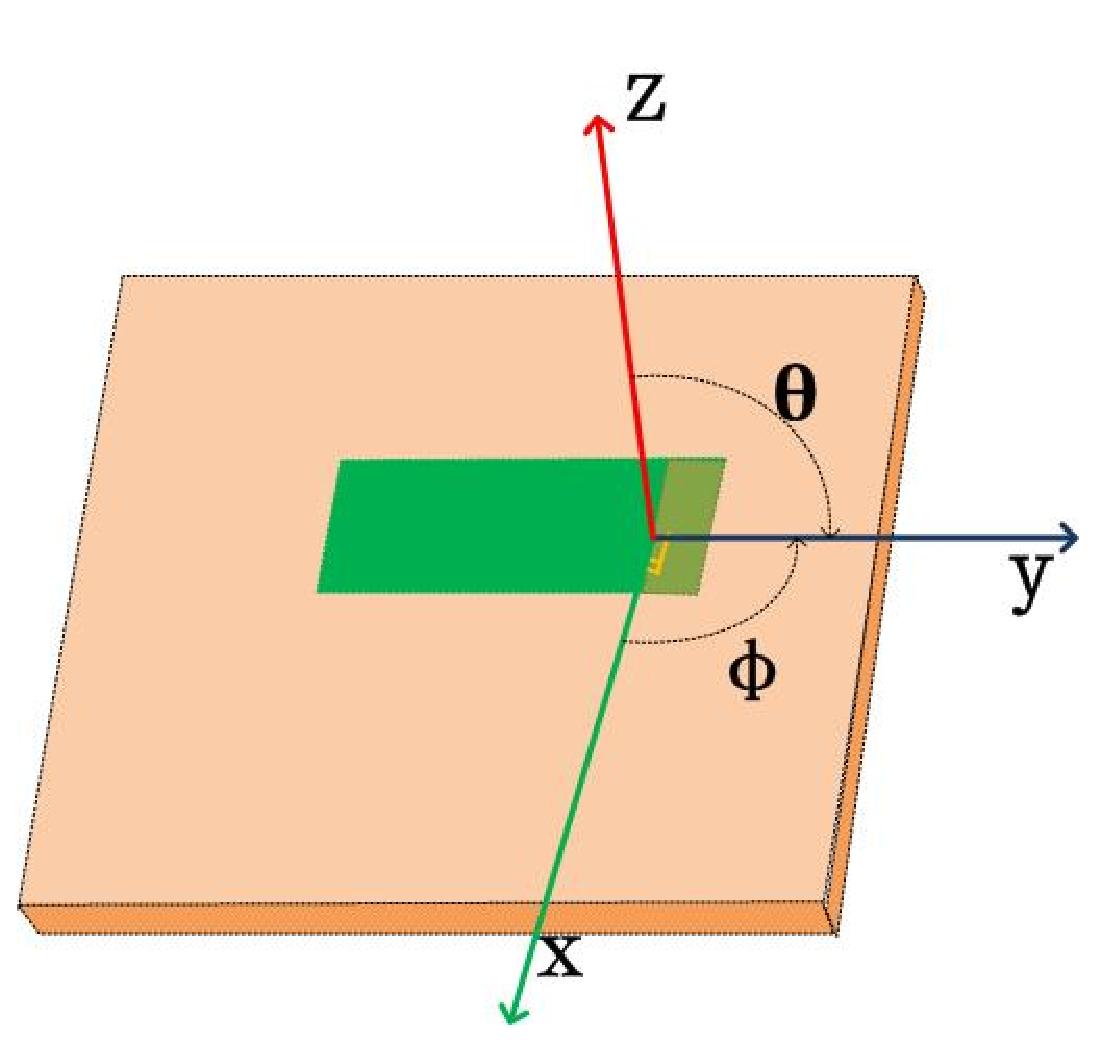
\includegraphics[width=\textwidth]{figs/5a.eps}
\caption{$S_{11}$ variation}
\label{fig:5a}	
\end{subfigure}		
\begin{subfigure}[b]{0.4\textwidth}
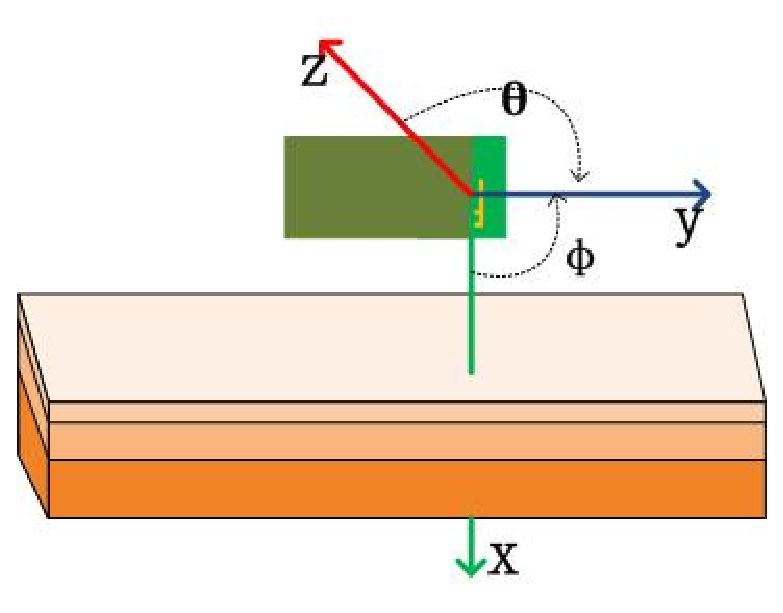
\includegraphics[width=\textwidth]{figs/5b.eps}
\caption{B variation}
\label{fig:5b}
\end{subfigure}
\caption{IFA: Comparison of $S_{11}$ and $B$ of horizontal polarization and vertical polarization with different $d$ }
\label{fig:5}
\end{figure}

\begin{figure}[!htb]
\centering
\begin{subfigure}[b]{0.22\textwidth}
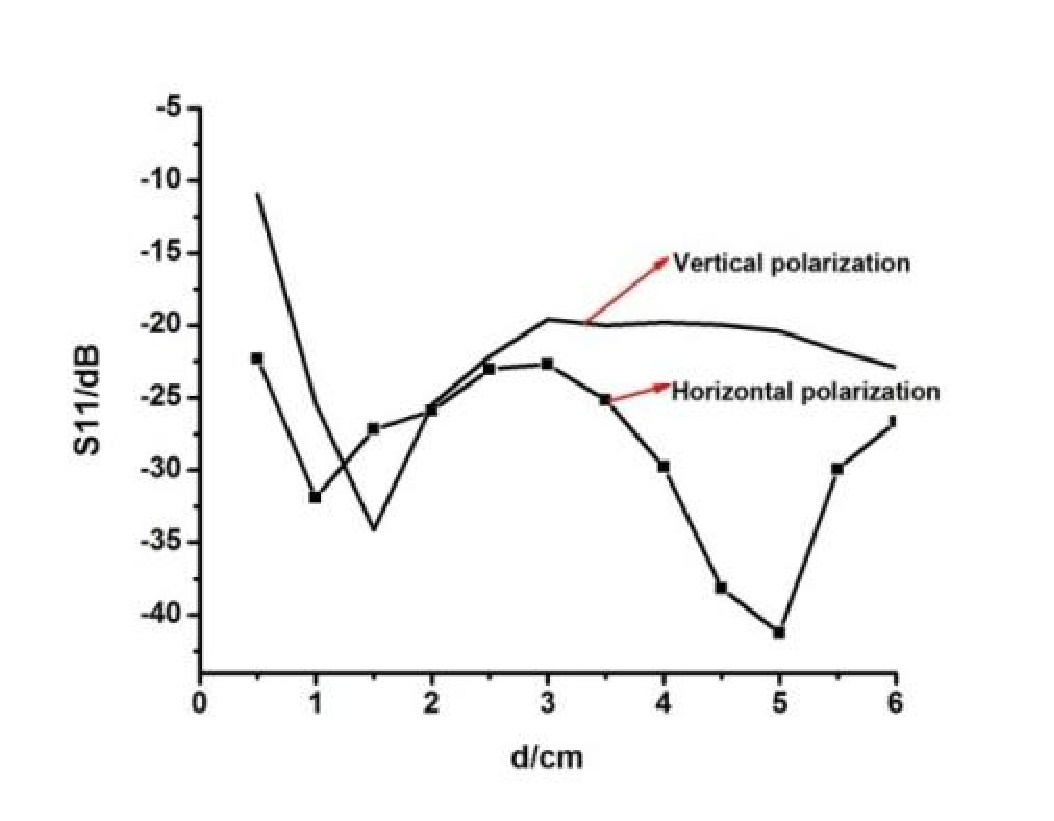
\includegraphics[width=\textwidth]{figs/6a.eps}
\caption{E-plane of horizontal polarization}
\label{fig:6a}	
\end{subfigure}		
\begin{subfigure}[b]{0.22\textwidth}
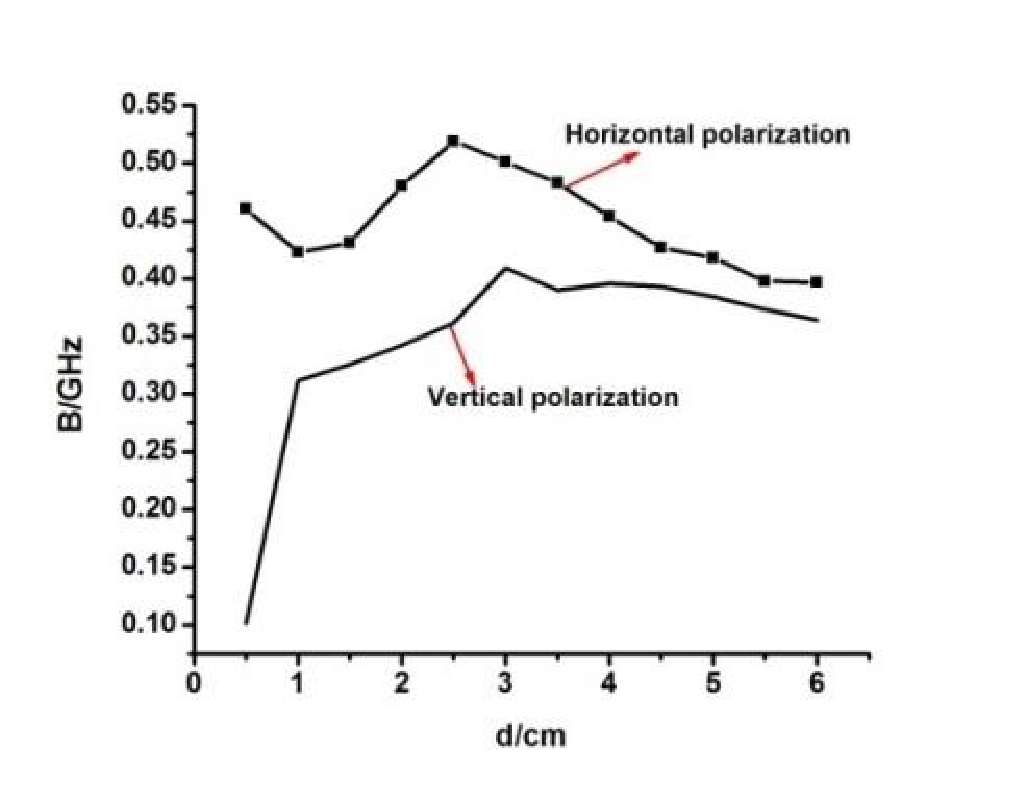
\includegraphics[width=\textwidth]{figs/6b.eps}
\caption{E-plane of vertical polarization}
\label{fig:6b}
\end{subfigure}
\begin{subfigure}[b]{0.22\textwidth}
\includegraphics[width=\textwidth]{figs/6e.eps}
\caption{H-plane of horizontal polarization}
\label{fig:6d}	
\end{subfigure}
\begin{subfigure}[b]{0.22\textwidth}
\includegraphics[width=\textwidth]{figs/6d.eps}
\caption{H-plane of vertical polarization}
\label{fig:6e}	
\end{subfigure}
\begin{subfigure}[b]{0.24\textwidth}
\includegraphics[width=\textwidth]{figs/6c.eps}
\caption{E-plane}
\label{fig:6c}	
\end{subfigure}
\begin{subfigure}[b]{0.24\textwidth}
\includegraphics[width=\textwidth]{figs/6f.eps}
\caption{H-plane}
\label{fig:6f}	
\end{subfigure}
\caption{IFA: Comparison of gain pattern of horizontal polarization and vertical polarization of $d$}.
$S^2= \frac{\sum_{d=1}^n{({G_b-G})^2}}{n}$ (d=1 cm, 2 cm, 4 cm, 6 cm) }
\label{fig:6}
\end{figure}

In horizontal polarization, the $S_{11}$ of the antenna decreases as $d$ increases. Consequently, the best antenna matching, i.e. the smallest $S_{11}$, is reached at $d=5 cm$.
In vertical polarization, $S_{11}$ shows unimodal distribution for 0.5 cm$<$d$<$4 cm, where its minimal value is observed at $d= 1.5 cm$.

In ranges 0.5 cm$<$d$<$1.2 cm and $d$$>$2 cm, the horizontal polarization of $S_{11}$ is always smaller than vertical polarization. It indicates that within these ranges, the IFA antenna in horizontal polarization will achieve better performance than in vertical polarization.

\begin{figure}[!htb]
\centering
\begin{subfigure}[b]{0.24\textwidth}
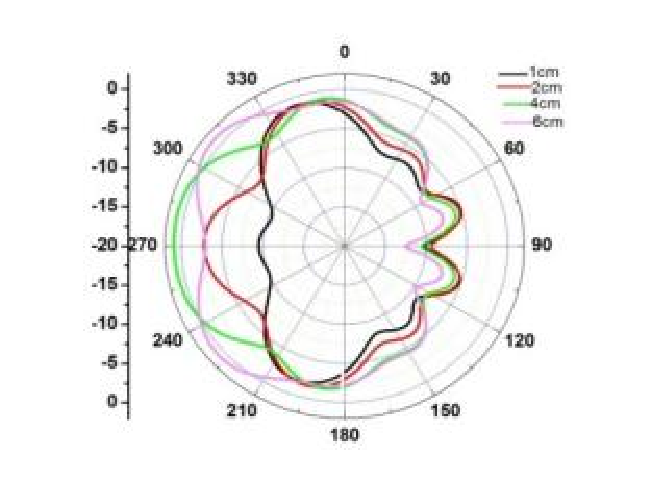
\includegraphics[width=\textwidth]{figs/7a.eps}
\caption{E-plane}
\label{fig:7a}	
\end{subfigure}
\begin{subfigure}[b]{0.24\textwidth}
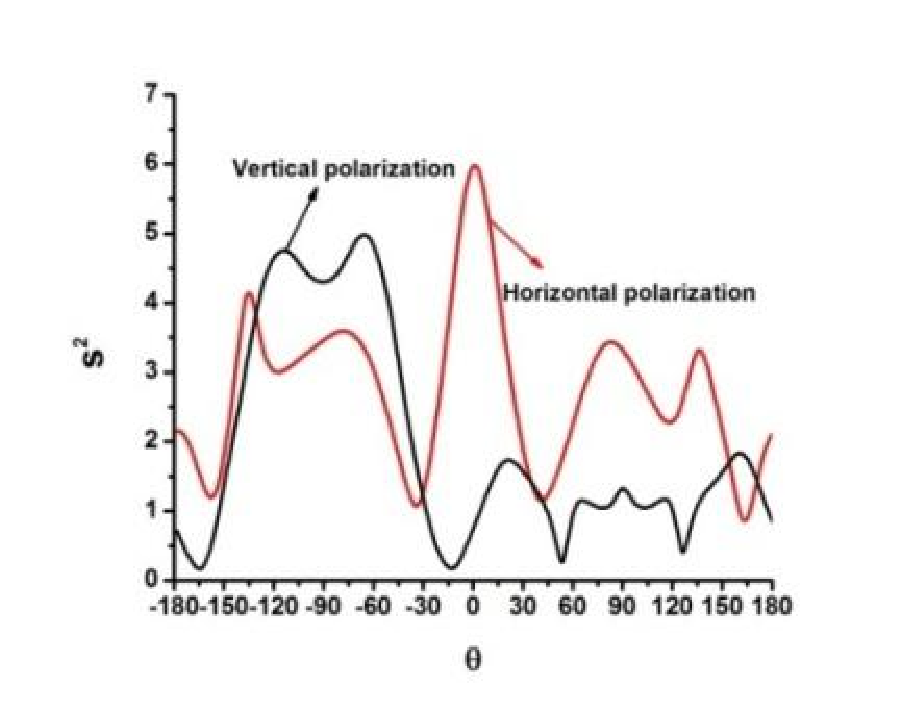
\includegraphics[width=\textwidth]{figs/7c.eps}
\caption{H-plane}
\label{fig:7c}	
\end{subfigure}		
\begin{subfigure}[b]{0.23\textwidth}
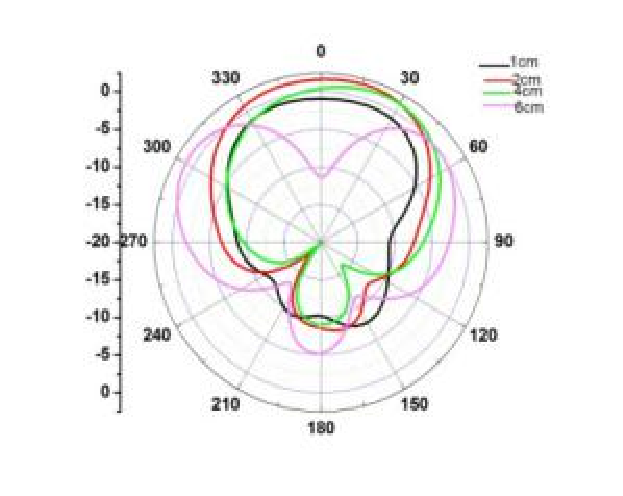
\includegraphics[width=\textwidth]{figs/7b.eps}
\caption{Differential gain of E-plane }
\label{fig:7b}
\end{subfigure}
\begin{subfigure}[b]{0.23\textwidth}

\includegraphics[width=\textwidth]{figs/7d.eps}
\caption{Differential gain of H-plane}
\label{fig:7d}	
\end{subfigure}
\caption{Gain pattern of IFA. $G_{b}$: Gain of antenna on body surface, $G_{f}$: Gain of antenna in free space }
\label{fig:7}
\end{figure}

Fig. \ref{fig:6} shows the radiation pattern of the IFA antennas in E-plane and H-plane respectively at different $d$.
As shown in Fig. \ref{fig:6}, the radiation pattern of the antenna in horizontal polarization at E-plane is stable and not sensitive to $d$ variation.
For For H-plane pattern, when $0\,^{\circ}$$<$ $\varphi$$<$$30\,^{\circ}$, $310\,^{\circ}$$<$ $\varphi$$<$$330\,^{\circ}$, $S^{2}$$>$5, indicating that the difference between the gain in the same direction is great and antenna directional gain is sensitive to $d$ .
The directional gain distribution of vertical polarization at different distances is uniform and not sensitive to the $d$. By comparing the antenna polarization performance at different distances, it is found that the impact on antenna is not significant for $d$ variation.

We then select $d = 5 cm$ and $d = 1.5 cm$ for horizontal polarization and vertical polarization, respectively, as the performance of the antenna is the best of these two distances. E-plane radiation pattern of horizontal polarization and vertical polarization after loading body model are symmetrical distribution of $\theta$=$0\,^{\circ}$ and $\theta$=$90\,^{\circ}$ as shown in Fig. \ref{fig:7}. The gain difference of horizontal polarization is described as Eq. \ref{eq:eps_2}

\begin{equation}
\label{eq:eps_2}
y[dB]=0.0003797x^2+0.00488x+1.00823  x[cm],
\end{equation}

The  body model has a great influence on the antenna gain at the position of $-180\,^{\circ}$$<$$\theta$$<$$-125\,^{\circ}$, $125\,^{\circ}$$<$$\theta$$<$$180\,^{\circ}$, and when $\theta$=$140\,^{\circ}$, $\mid$$G_{b}$-$G_{f}$$\mid$ is the maximum and the human body has the most obvious effects on antenna. For vertical polarization, $\mid$$G_{b}$-$G_{f}$$\mid$$<$6 dB, human body has a uniform effect on antenna gain pattern over the entire range of $\theta$. The impact of human body to vertical polarization are more obvious than horizontal polarization.

H-plane pattern of horizontal polarization after loading body model is similar to omnidirectional distribution of free
space. For vertical polarization, when $0\,^{\circ}$$<$ $\varphi$$<$$35\,^{\circ}$, $295\,^{\circ}$$<$
$\varphi$$<$$320\,^{\circ}$, $340\,^{\circ}$$<$ $\varphi$$<$$360\,^{\circ}$, $\mid$$G_{b}$-$G_{f}$$\mid$$>$4 dB, human
body has great effects on antenna gain pattern, when $\varphi$=$17\,^{\circ}$, $\mid$$G_{b}$-$G_{f}$$\mid$ reach the
maximum and human body has the most obvious effects on antenna.

\subsection{MIFA}
\begin{figure}[!htb]
\centering
\begin{figure}[!htb]
\centering
\begin{subfigure}[b]{0.4\textwidth}
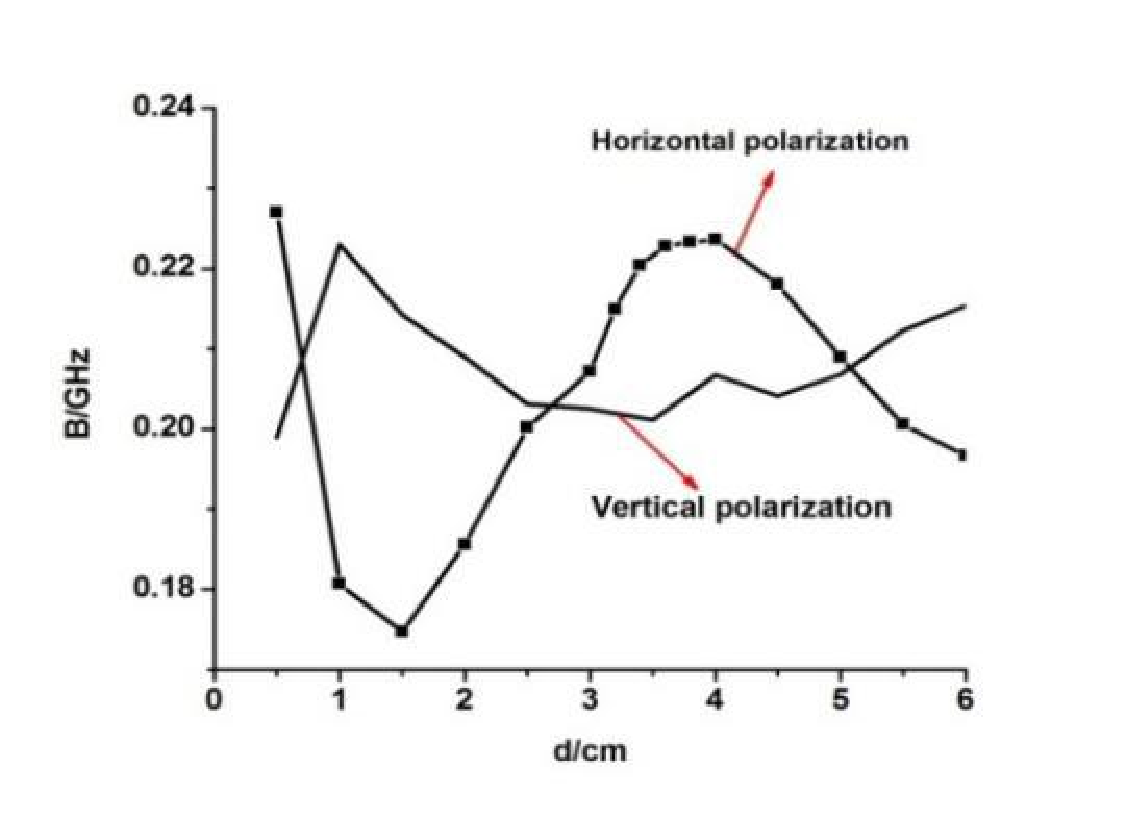
\includegraphics[width=\textwidth]{figs/8a.eps}
\caption{$S_{11}$ variation}
\label{fig:8a}	
\end{subfigure}		
\begin{subfigure}[b]{0.4\textwidth}
\includegraphics[width=\textwidth]{figs/8b.eps}
\caption{$B$ variation}
\label{fig:8b}
\end{subfigure}
\caption{MIFA: Comparison of $S_{11}$ and B of horizontal polarization and vertical polarization with different $d$ }
\label{fig:8}
\end{figure}

For horizontal polarization, the effect of distance on bandwidth is not obvious. The bandwidth approximated by Eq. \ref{eq:eps_3}. When $d$=1.5 cm, the bandwidth is the narrowest, and the antenna is not suitable for placing on body surface. When $d$=0.5 cm and $d$=4 cm, $B$=225 GHz, reaching the maximum. When $d$=1 cm, the bandwidth of vertical polarization is the narrowest, so the antenna is not suitable for placing on human body surface.

 \begin{equation}
\label{eq:eps_3}
y[GHz]=-0.00178x^2+0.01416x+0.18396,  x[cm]
\end{equation}

\begin{equation}
\label{eq:eps_4}
y[dB]=2.02866x-16.01,  x[cm]
\end{equation}

\begin{figure}[!htb]
\centering
\begin{subfigure}[b]{0.24\textwidth}
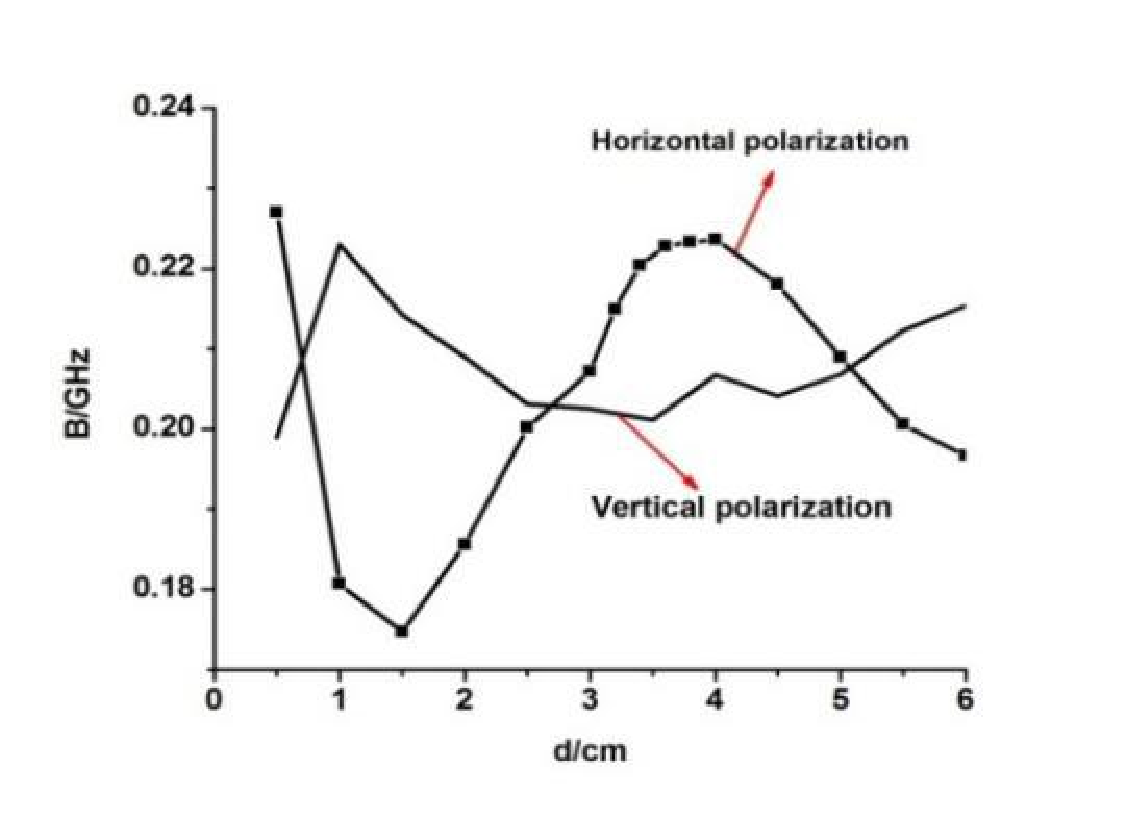
\includegraphics[width=\textwidth]{figs/9a.eps}
\caption{Horizontal polarization of E-plane}
\label{fig:9a}	
\end{subfigure}		
\begin{subfigure}[b]{0.24\textwidth}
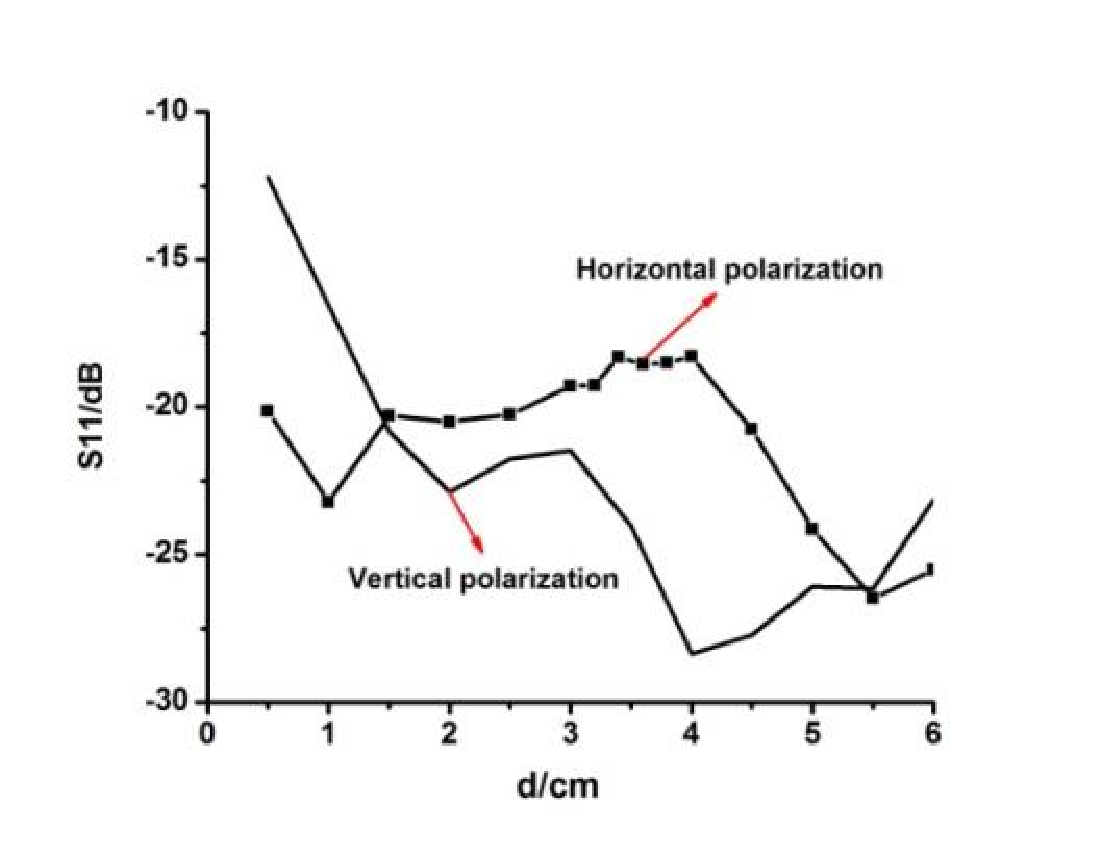
\includegraphics[width=\textwidth]{figs/9b.eps}
\caption{Vertical polarization of E-plane }
\label{fig:9b}
\end{subfigure}
\begin{subfigure}[b]{0.24\textwidth}
\includegraphics[width=\textwidth]{figs/9d.eps}
\caption{Horizontal polarization of H-plane}
\label{fig:9d}	
\end{subfigure}
\begin{subfigure}[b]{0.24\textwidth}
\includegraphics[width=\textwidth]{figs/9e.eps}
\caption{Vertical polarization of H-plane}
\label{fig:9e}	
\end{subfigure}
\begin{subfigure}[b]{0.24\textwidth}
\includegraphics[width=\textwidth]{figs/9c.eps}
\caption{E-plane}
\label{fig:9c}	
\end{subfigure}
\begin{subfigure}[b]{0.24\textwidth}
\includegraphics[width=\textwidth]{figs/9f.eps}
\caption{H-plane}
\label{fig:9f}	
\end{subfigure}
\caption{MIFA: Comparison of gain pattern of horizontal polarization and vertical polarization of $d$}
\label{fig:9}
\end{figure}

The equation of $S_{11}$ variation in vertical polarization is given in Eq. \ref{eq:eps_4}. The minimal $S_{11}$ of the MIFA antennas is observed at $d$= 5.5 cm and when $d$=0.5cm, $S_{11}$ take the maximum. The $S_{11}$ curve of horizontal polarization is flat and when $d$=4 cm, $B$ reaches the maximum, so the antenna is most suitable to place on human body surface.

In the range of 1.5 cm$<$$d$$<$3 cm, $S_{11}$ of vertically polarized is always smaller than horizontal polarization, and the bandwidth is always wider than horizontal polarization. In this range, the antenna is more suitable for placing on the surface of the human body in vertically polarized.

In horizontal polarization, the standard deviation (STD) of the radiation gain are uniformly distributed as shown in Fig. \ref{fig:10}, showing insensitivity to $d$.

For E-plane pattern of vertical polarization, when $30\,^{\circ}$$<$$\varphi$$<$$150\,^{\circ}$, when $30\,^{\circ}$$<$$\varphi$$<$$150\,^{\circ}$, $S^{2}$$>$4, The gain difference at different distances is relatively large, the antenna direction gain is more sensitive to the distance factor than the other position.
For H-plane pattern, when $130\,^{\circ}$$<$ $\varphi$$<$$180\,^{\circ}$, $0\,^{\circ}$$<$ $\varphi$$<$$30\,^{\circ}$, $225\,^{\circ}$$<$ $\varphi$$<$$240\,^{\circ}$, $330\,^{\circ}$$<$ $\varphi$$<$$360\,^{\circ}$, $S^{2}$$>$4, the antenna direction gain is more sensitive to the distance factor.

\begin{figure}[!htb]
\centering
\begin{subfigure}[b]{0.24\textwidth}
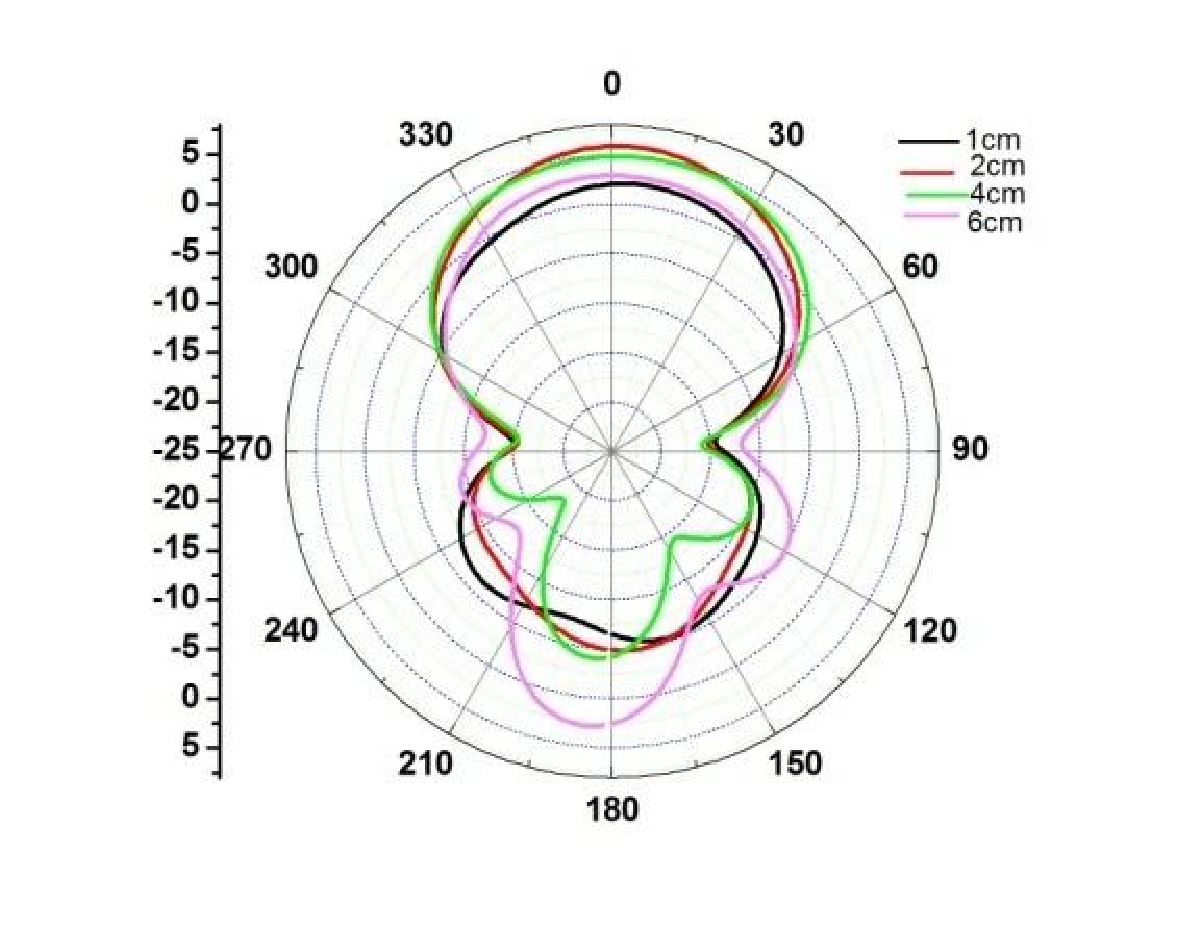
\includegraphics[width=\textwidth]{figs/10a.eps}
\caption{E-plane}
\label{fig:10a}	
\end{subfigure}		
\begin{subfigure}[b]{0.24\textwidth}
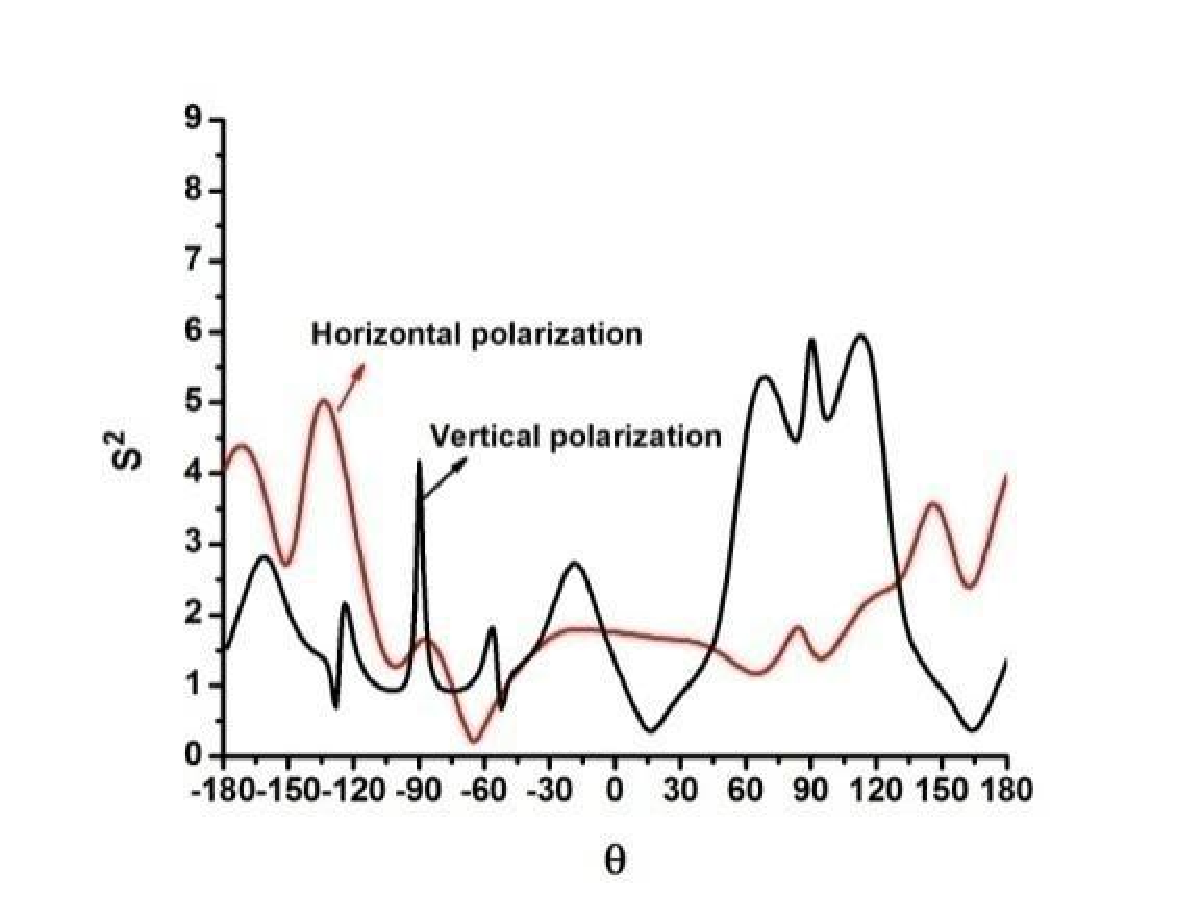
\includegraphics[width=\textwidth]{figs/10c.eps}
\caption{H-plane}
\label{fig:10c}	
\end{subfigure}
\begin{subfigure}[b]{0.24\textwidth}
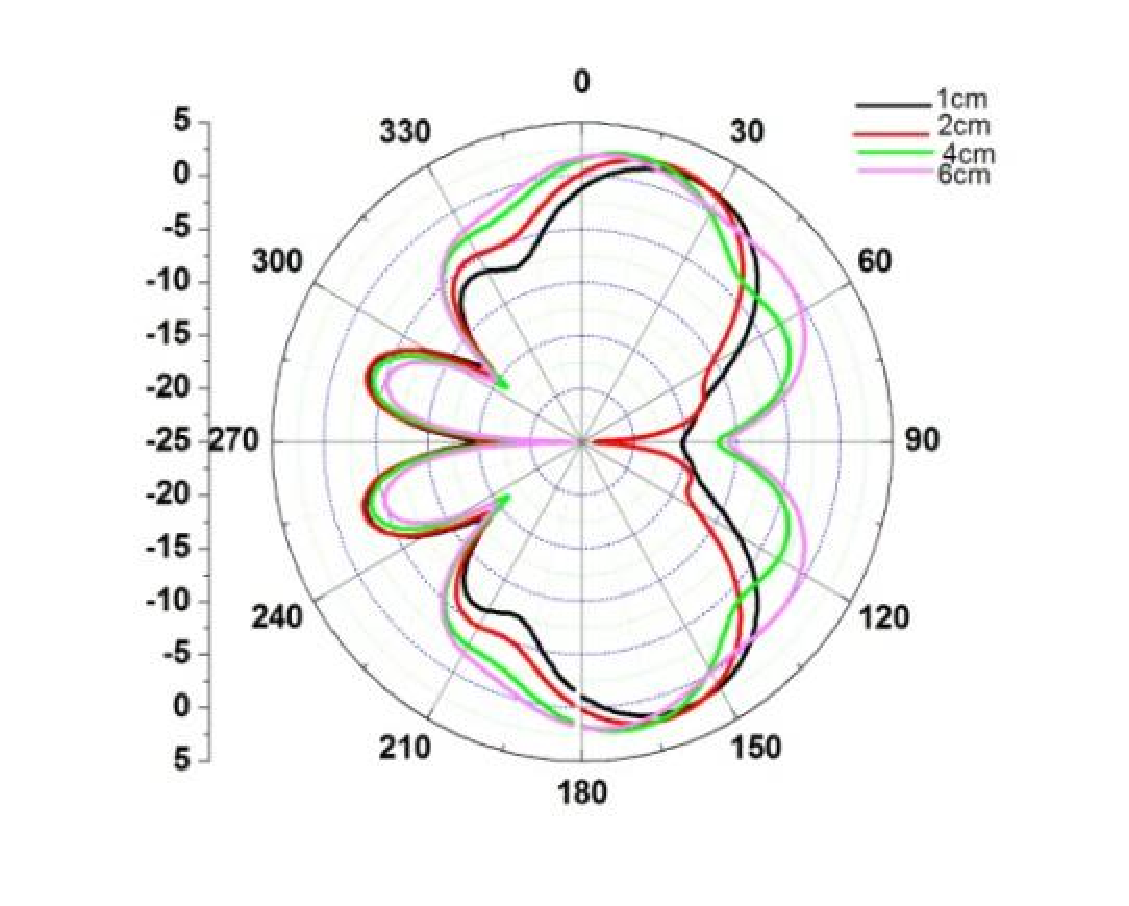
\includegraphics[width=\textwidth]{figs/10b.eps}
\caption{Differential gain of E-plane }
\label{fig:10b}
\end{subfigure}
\begin{subfigure}[b]{0.24\textwidth}
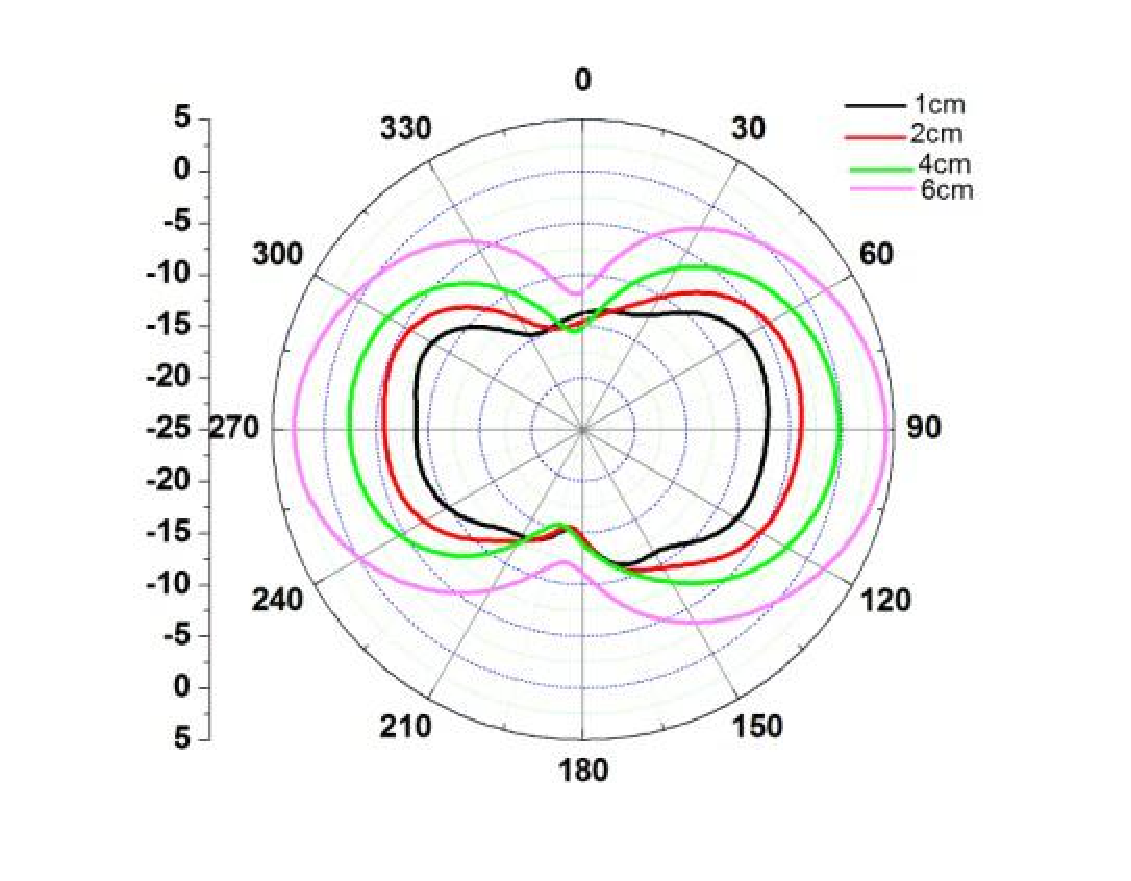
\includegraphics[width=\textwidth]{figs/10d.eps}
\caption{Differential gain of H-plane}
\label{fig:10d}	
\end{subfigure}
\caption{Radiation pattern of MIFA}
\label{fig:10}
\end{figure}

Fig. \ref{fig:9} shows the radiation pattern of the antenna in free space and after loading body model. Horizontal
polarization and vertical polarization were selected  $d$ = 5.5 cm and  $d$ = 4 cm respectively as the research focus. The antenna radiation  pattern of horizontal polarization and vertical polarization after loading human body model is symmetrically distributed with $\theta$=$0\,^{\circ}$ and $90\,^{\circ}$, respectively. The gain difference of horizontal polarization is described by Eq. \ref{eq:eps_5}.

\begin{equation}
\label{eq:eps_5}
y[dB]=-4.5676x^2-0.0018x+1.1592, x[cm]
\end{equation}

For E-plane radiation pattern of horizontal polarization, at the position of $-180\,^{\circ}$$<$$\theta$$<$$-110\,^{\circ}$, $110\,^{\circ}$$<$$\theta$$<$$180\,^{\circ}$, $\mid$$G_{b}$-$G_{f}$$\mid$$>$4 dB, the human body has a significant effect on antenna gain pattern. When $\theta$=$150\,^{\circ}$, $\mid$$G_{b}$-$G_{f}$$\mid$ takes the maximum, the human body has the greatest effect on antenna gain pattern.
For vertical polarization, at the position of $-135\,^{\circ}$$<$$\theta$$<$$120\,^{\circ}$, $-65\,^{\circ}$$<$$\theta$$<$$-45\,^{\circ}$, $\mid$$G_{b}$-$G_{f}$$\mid$$>$6 dB, the effect of the body on antenna gain
pattern is obvious, when $\theta$=$130\,^{\circ}$ and $\theta$=$550\,^{\circ}$, $\mid$$G_{b}$-$G_{f}$$\mid$=12 dB, reaches
the maximum, human body has the greatest effect on antenna gain pattern.

For H-plane gain pattern of the horizontal polarization, the gain curve is always smooth and the body has negligible effect
on the antenna gain pattern. For vertical polarization, the curve fluctuates obviously at the position of
$145\,^{\circ}$$<$$\theta$$<$$230\,^{\circ}$, $\mid$$G_{b}$-$G_{f}$$\mid$ takes the maximum and the human body has the most obvious effect on antenna.

\subsection{Printed dipole}

\begin{figure}[!htb]
\centering
\begin{subfigure}[b]{0.4\textwidth}
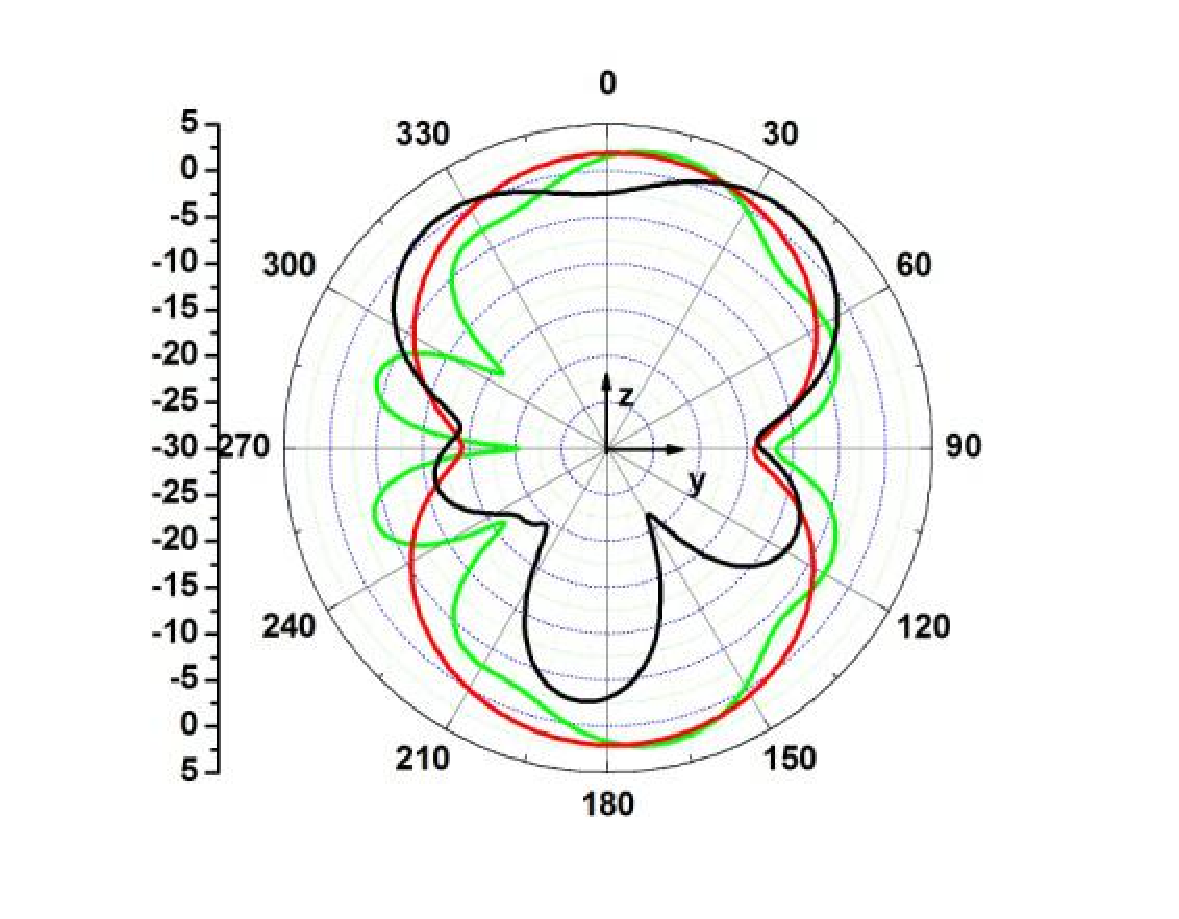
\includegraphics[width=\textwidth]{figs/11a.eps}
\caption{$S_{11}$ variation}
\label{fig:11a}	
\end{subfigure}		
\begin{subfigure}[b]{0.4\textwidth}
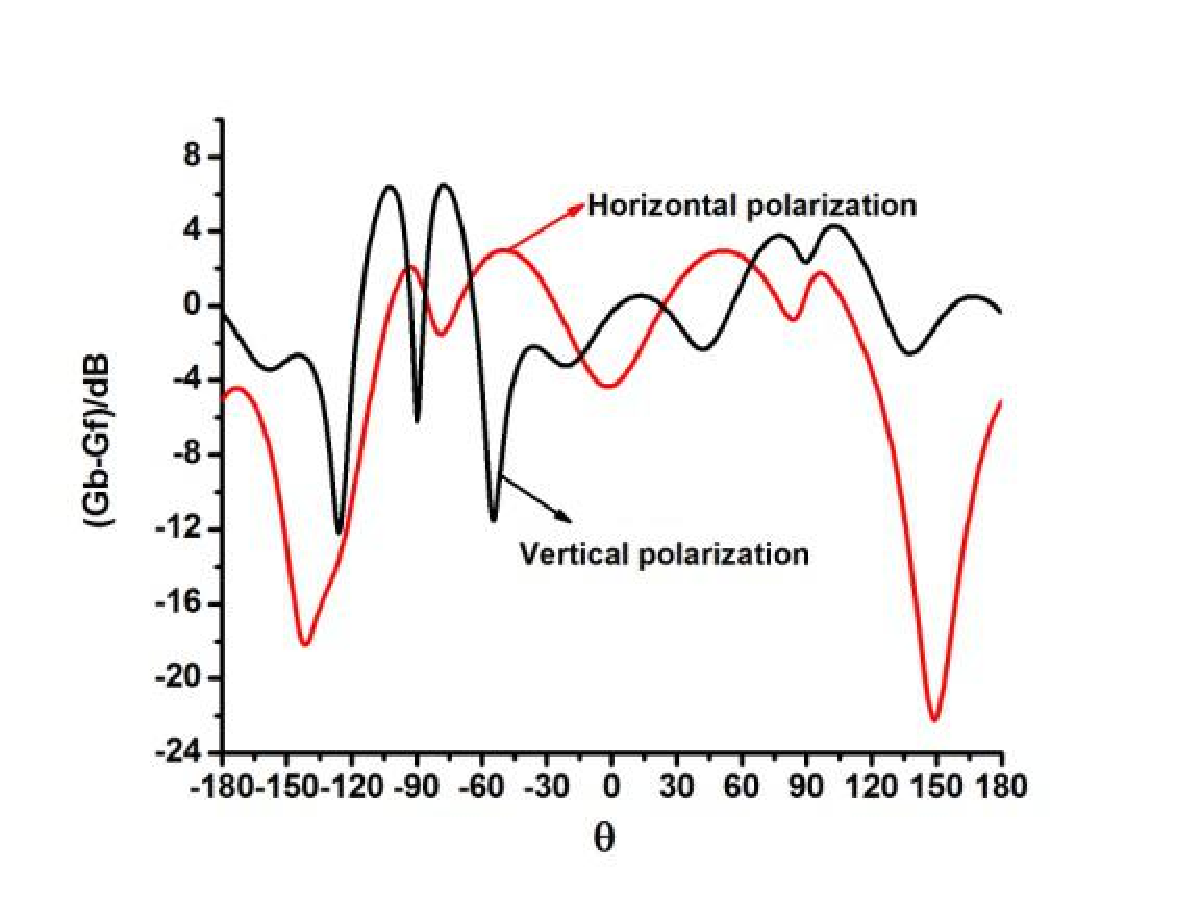
\includegraphics[width=\textwidth]{figs/11b.eps}
\caption{$B$ variation}
\label{fig:11b}
\end{subfigure}
\caption{Dipole: Comparison of $S_{11}$ and B of horizontal polarization and vertical polarization with different $d$}
\label{fig:11}
\end{figure}

Fig. \ref{fig:11} shows the changes of antenna matching performance and bandwidth of $d$. In horizontal polarization, the bandwidth of dipole antenna is described as Eq. \ref{eq:eps_6}. The minimal bandwidth is observed at $d$=1 cm and the antenna is not suitable for placing on body surface. In vertical polarization, the bandwidth variation curve is always smooth and the body has negligible effect on the antenna. It is approximated by Eq. \ref{eq:eps_7}.

We can see form the $S_{11}$ curve shown in Eq. \ref{eq:eps_7}, the trend of vertical polarization and horizontal polarization is consistent. In horizontal polarization, the minimal $S_{11}$ of the dipole antennas is observed at $d$= 5.5 cm and when the antenna placed 3 cm from the body surface in vertical polarization, the antenna performance is the best. $S_{11}$ of horizontal polarization is always greater than vertical polarization. When 0 cm$<$$d$$<$3 cm, the bandwidth of
vertical polarization is always greater than horizontal Polarization. Therefore, in this range of $d$, the antenna is
more suitable for vertical polarization.

\begin{equation}
\label{eq:eps_6}
y[dB]=0.014x+0.4937, x[cm]
\end{equation}

\begin{equation}
\label{eq:eps_7}
y[dB]=-0.0153x^2-0.2802x+0.52222, x[cm]
\end{equation}

\begin{equation}
\label{eq:eps_8}
y[dB]=-0.838x-37.197, x[cm]
\end{equation}
\begin{equation}
\label{eq:eps_9}
y[dB]=-3.4777x-12.723, x[cm]
\end{equation}

\begin{figure}[!htb]
\centering
\begin{subfigure}[b]{0.24\textwidth}
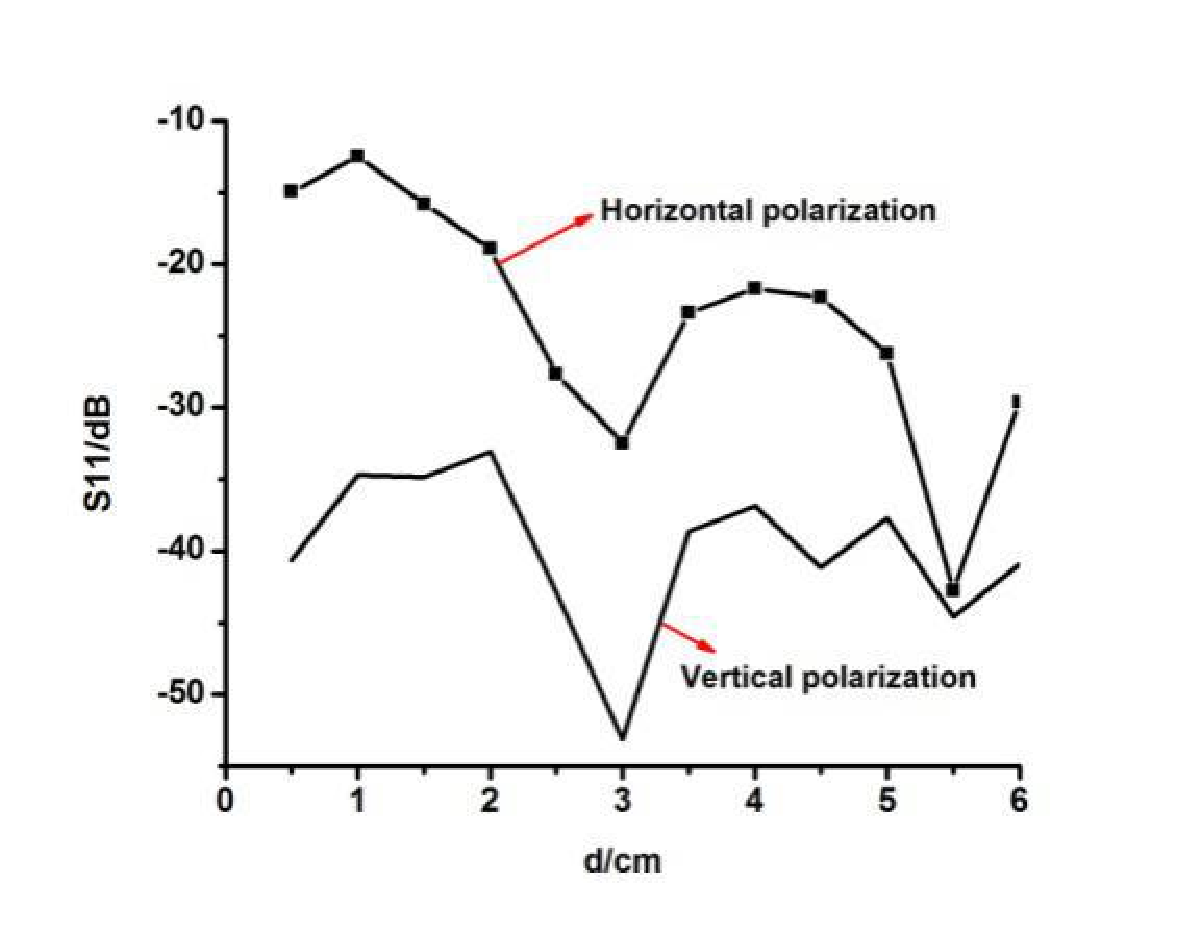
\includegraphics[width=\textwidth]{figs/12a.eps}
\caption{Horizontal polarization of E-plane}
\label{fig:12a}	
\end{subfigure}		
\begin{subfigure}[b]{0.24\textwidth}
\includegraphics[width=\textwidth]{figs/12d.eps}
\caption{Horizontal polarization H-plane}
\label{fig:12d}	
\end{subfigure}
\begin{subfigure}[b]{0.24\textwidth}
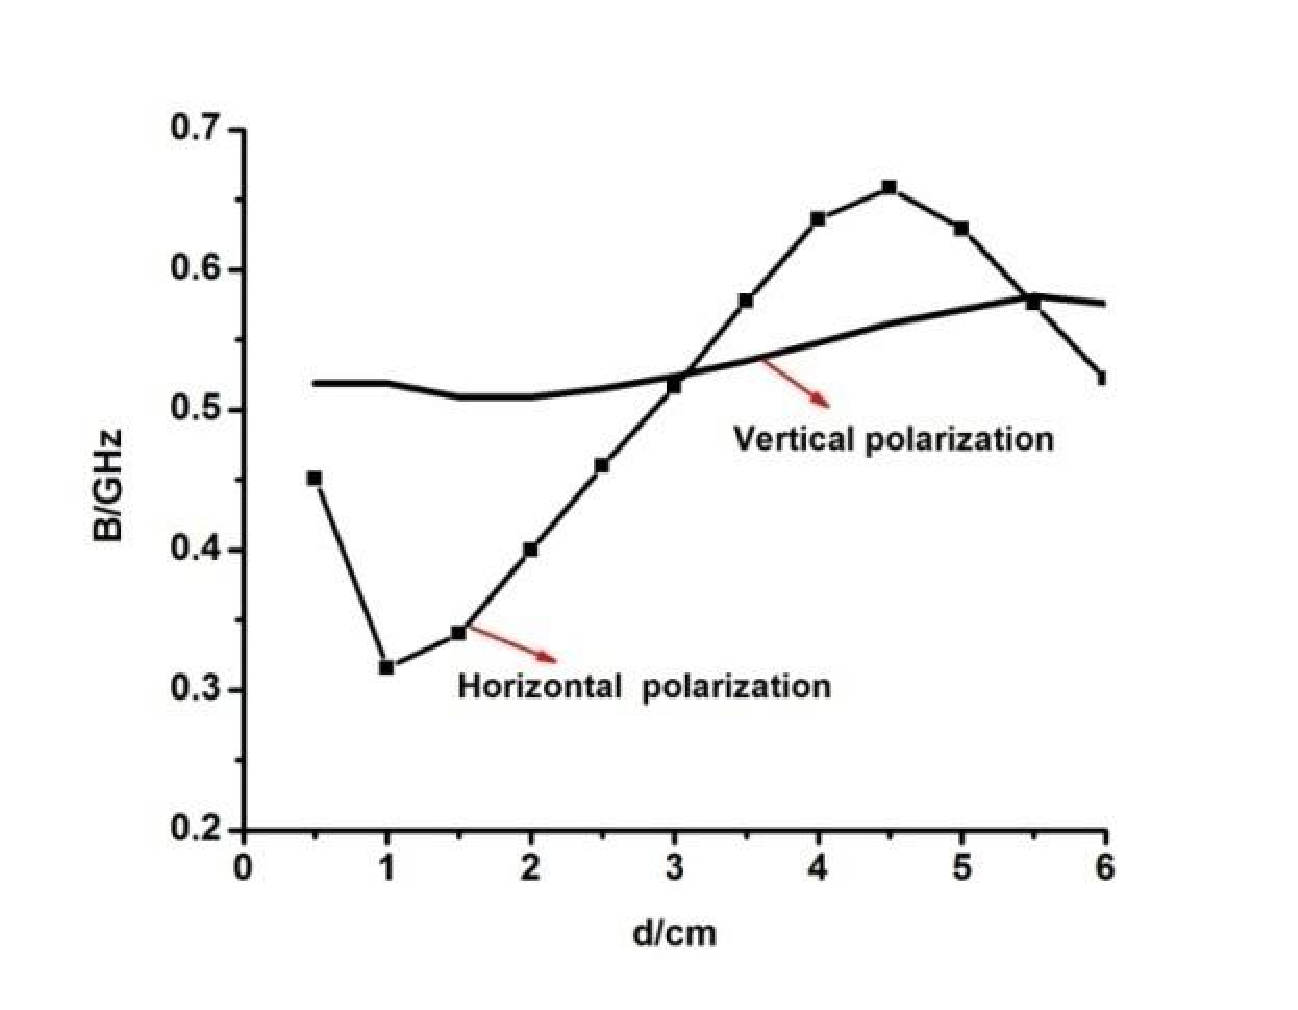
\includegraphics[width=\textwidth]{figs/12b.eps}
\caption{Vertical polarization E-plane}
\label{fig:12b}
\end{subfigure}
\begin{subfigure}[b]{0.24\textwidth}
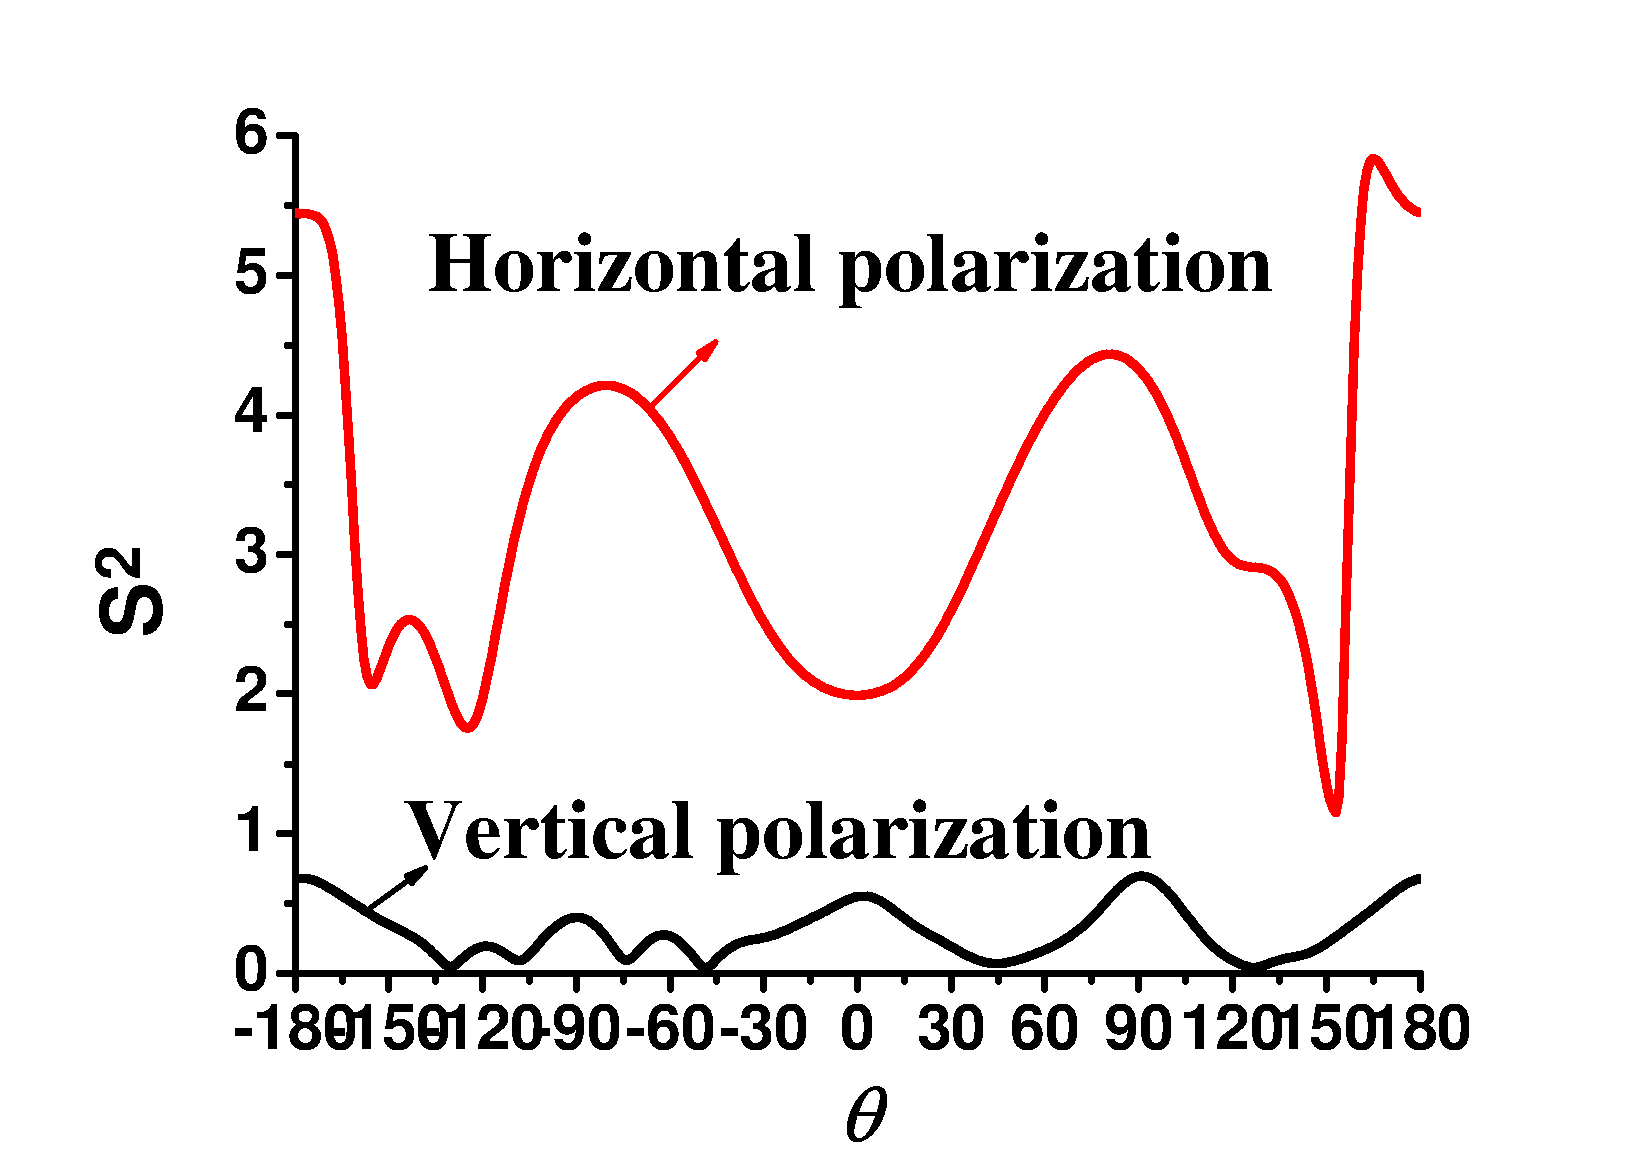
\includegraphics[width=\textwidth]{figs/12e.eps}
\caption{Vertical polarization of H-plane}
\label{fig:12e}	
\end{subfigure}
\begin{subfigure}[b]{0.24\textwidth}
\includegraphics[width=\textwidth]{figs/12c.eps}
\caption{E-plane}
\label{fig:12c}	
\end{subfigure}
\begin{subfigure}[b]{0.24\textwidth}
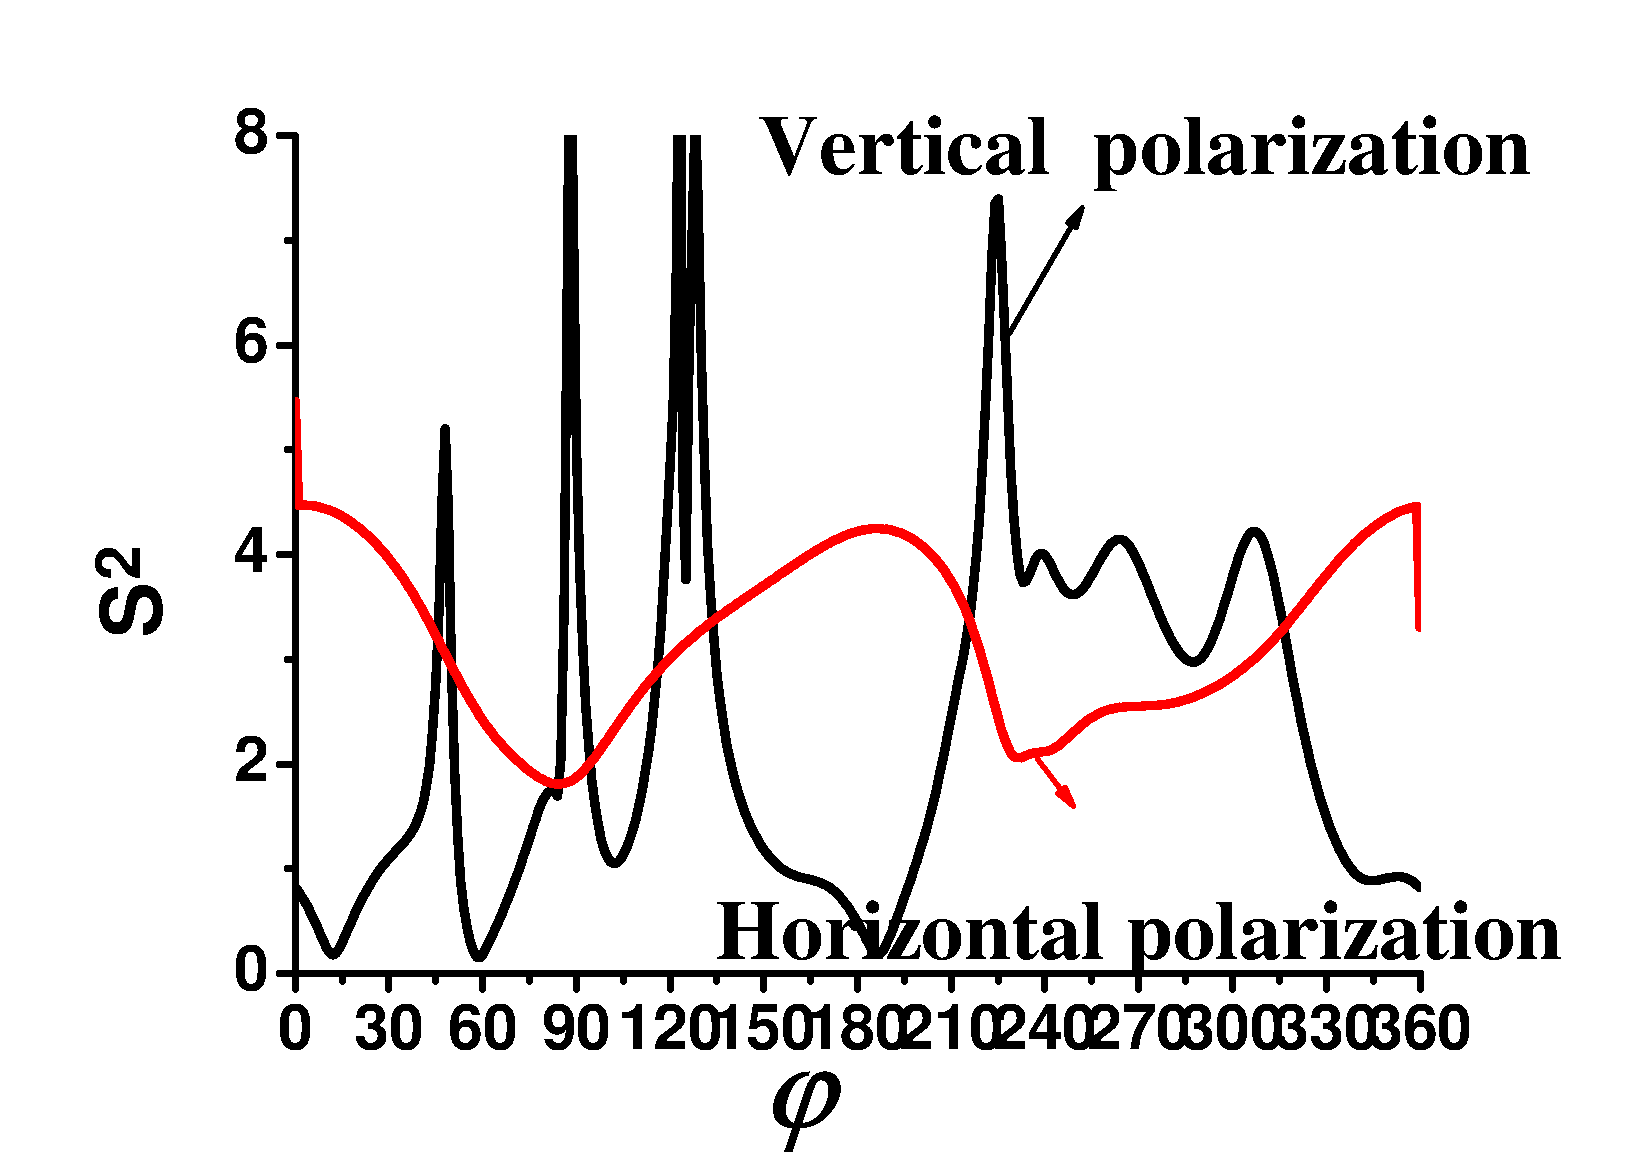
\includegraphics[width=\textwidth]{figs/12f.eps}
\caption{H-plane}
\label{fig:12f}	
\end{subfigure}
\caption{Dipole: Comparison of gain pattern of horizontal polarization and vertical polarization of $d$}
\label{fig:12}
\end{figure}

For horizontal polarization as shown in fig. \ref{fig:12a} and fig. \ref{fig:12d}. The standard deviation (STD) of the radiation gain are uniformly distributed, showing insensitivity to $d$. In vertical polarization shown in fig. \ref{fig:12b} and fig. \ref{fig:12e}, at the position of $85\,^{\circ}$$<$$\varphi$$<$$90\,^{\circ}$, $120\,^{\circ}$$<$$\varphi$$<$$130\,^{\circ}$, $220\,^{\circ}$$<$$\varphi$$<$$230\,^{\circ}$, $S^{2}$$>$7, the
difference of H-plane pattern of $d$ is relatively great, the antenna direction gain is more sensitive to $d$.

\begin{figure}[!htb]
\centering
\begin{subfigure}[b]{0.24\textwidth}
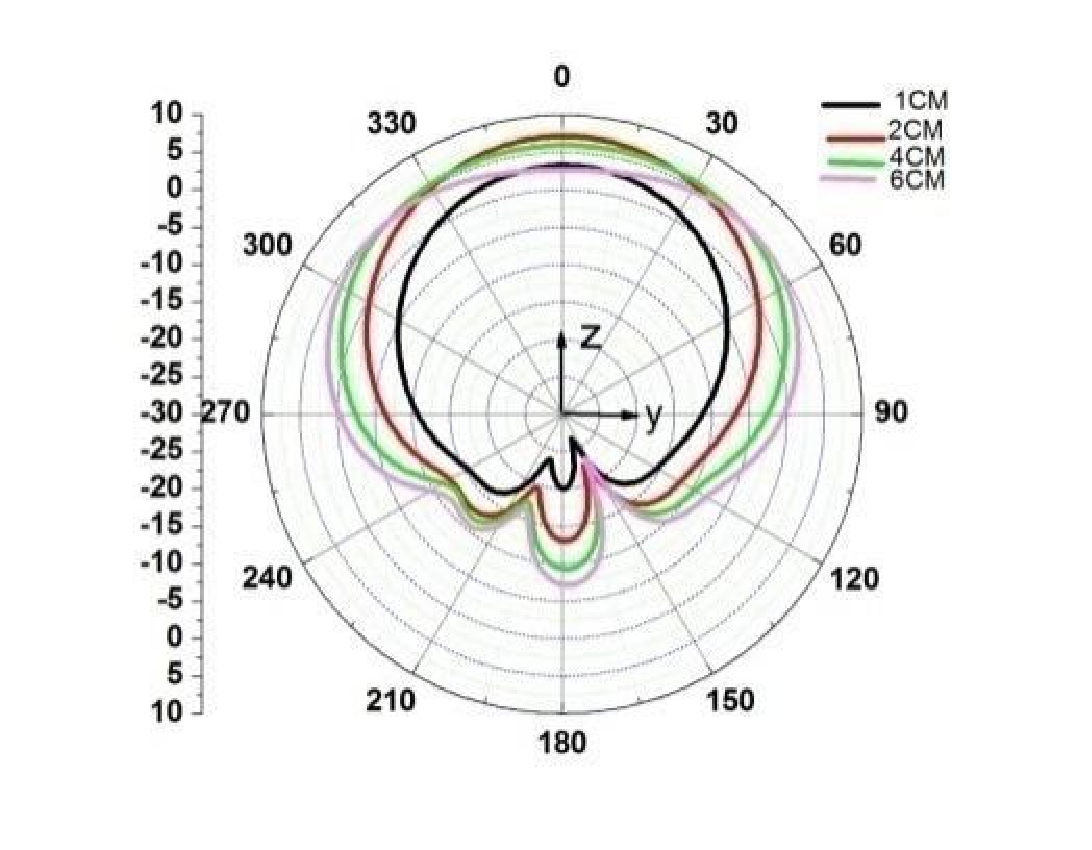
\includegraphics[width=\textwidth]{figs/13a.eps}
\caption{E-plane}
\label{fig:a}	
\end{subfigure}		
\begin{subfigure}[b]{0.24\textwidth}
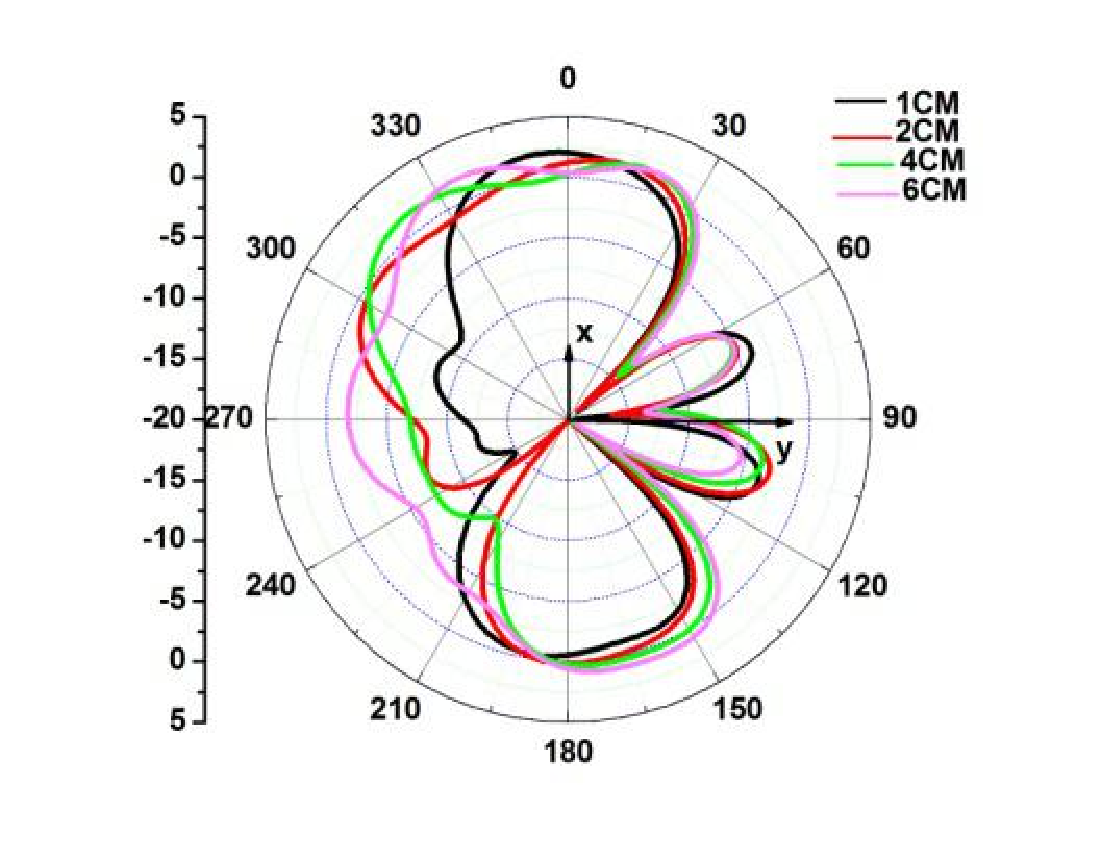
\includegraphics[width=\textwidth]{figs/13b.eps}
\caption{H-plane}
\label{fig:c}	
\end{subfigure}
\begin{subfigure}[b]{0.24\textwidth}
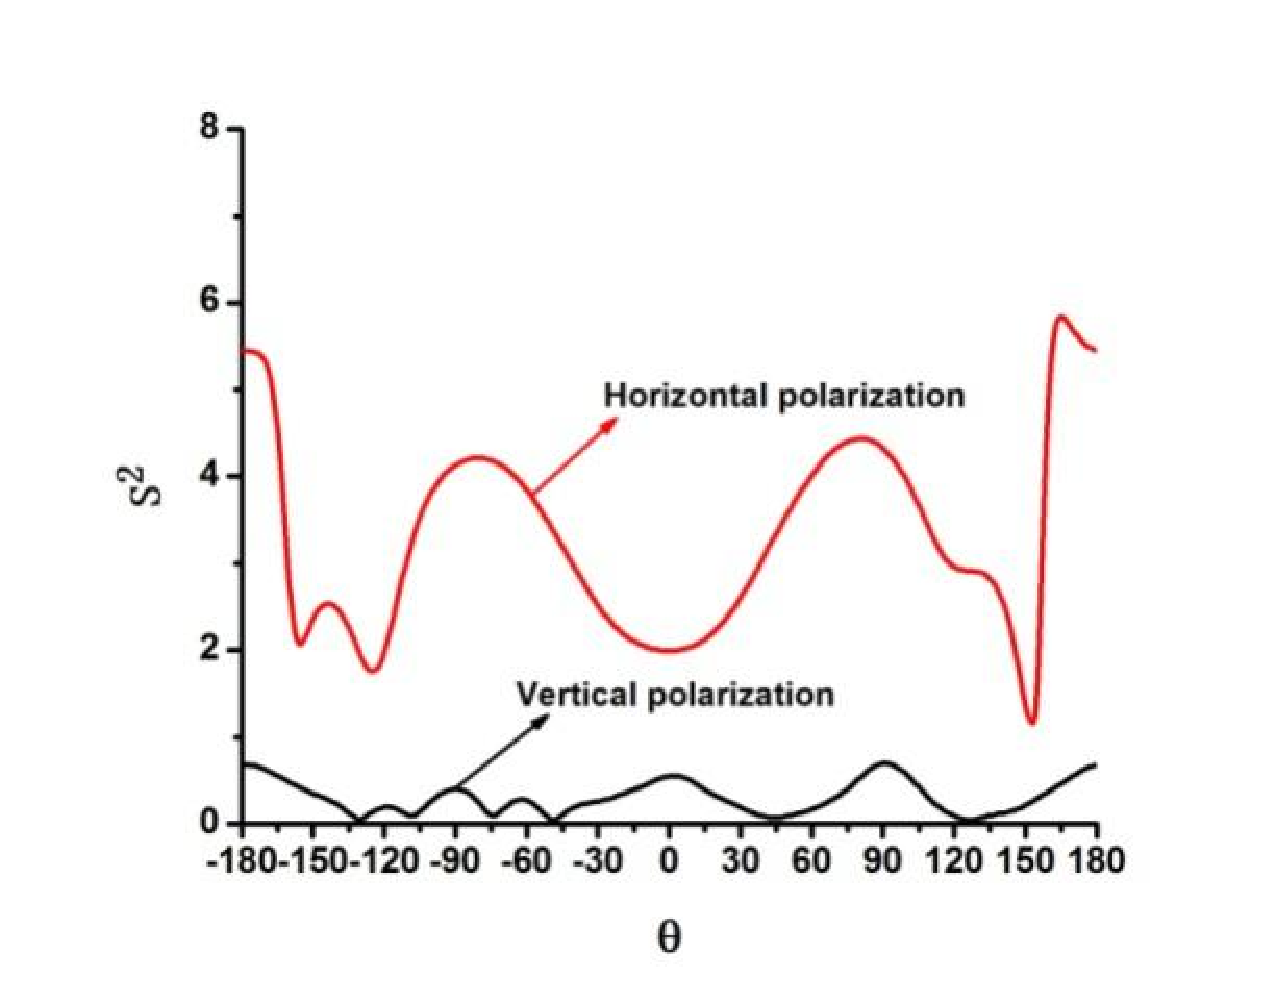
\includegraphics[width=\textwidth]{figs/13c.eps}
\caption{Differential gain of E-plane }
\label{fig:b}
\end{subfigure}
\begin{subfigure}[b]{0.24\textwidth}
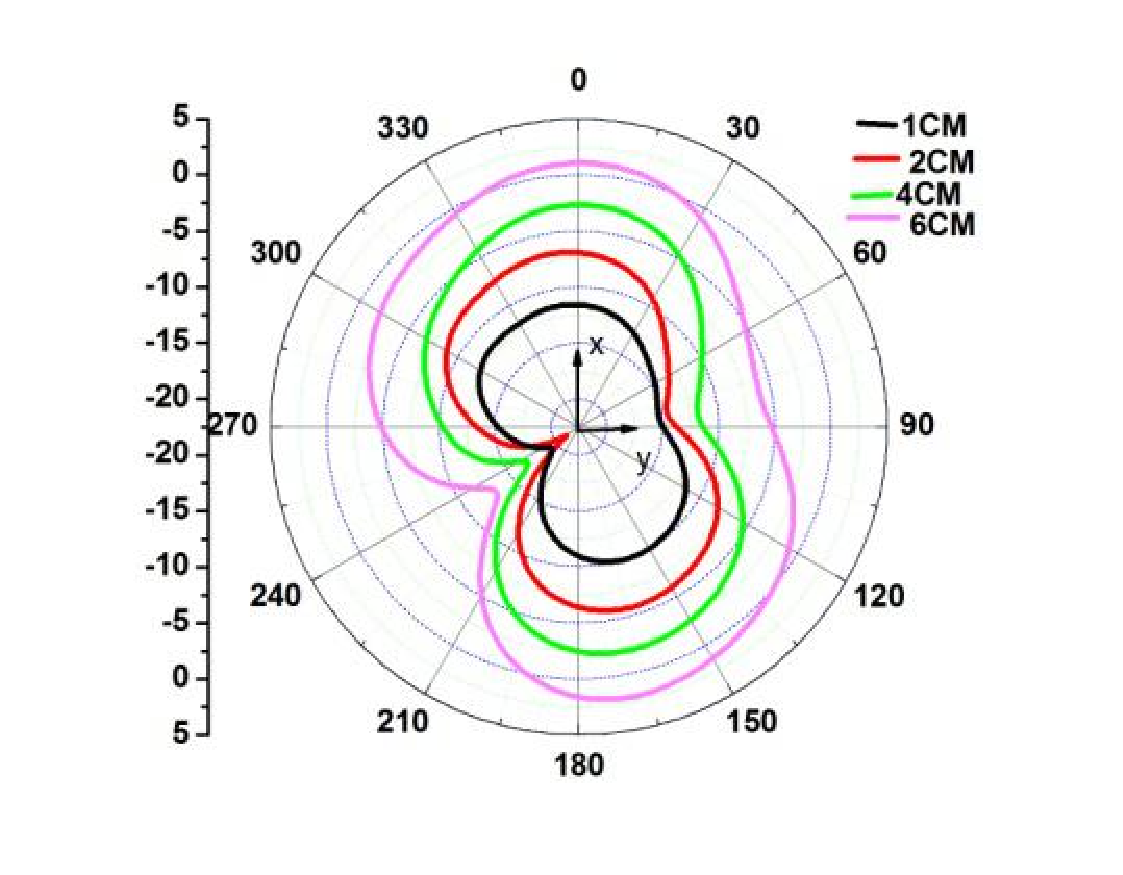
\includegraphics[width=\textwidth]{figs/13d.eps}
\caption{Differential gain of H-plane}
\label{fig:d}	
\end{subfigure}
\caption{Radiation pattern of dipole}
\label{fig:13}
\end{figure}

Horizontal polarization and vertical polarization were selected $d$=5.5 cm and $d$=3 cm as the focus of research, respectively. The dipole antenna performance of this $d$ is better and antenna radiation orientation is more obvious than the other $d$, the maximum gain reached 5 dB.

E-plane radiation pattern of horizontal polarization and vertical polarization after loading body model are symmetrical distribution of $\theta$=$0\,^{\circ}$ and $\theta$=$90\,^{\circ}$ as shown in Fig. \ref{fig:13}. E-plane pattern of vertical polarization after loading the human body is close to omnidirectional distribution of free space.
For horizontal polarization, the gain difference approximated by Eq. \ref{eq:eps_10}.

\begin{equation}
\label{eq:eps_10}
y[dB]=-0.0006078x^2-0.00243x+2.26111, x[cm]
\end{equation}

For E-plane radiation pattern of dipole antenna in horizontal polarization, due to the radiation of human body, at the position of $130\,^{\circ}$$<$$\theta$$<$$180\,^{\circ}$ and $-130\,^{\circ}$$<$$\theta$$<$$-180\,^{\circ}$, the gain difference is relatively great and the human body has obvious effect on antenna gain pattern. The gain is enhanced at the position of $-90\,^{\circ}$$<$$\theta$$<$$-15\,^{\circ}$ and weakened at the other position.
For H-plane radiation pattern of horizontal polarization, $\mid$$G_{b}$-$G_{f}$$\mid$$<$4 dB, the body has negligible effect on the antenna gain pattern.

For E-plane radiation pattern of dipole antenna in vertical polarization, the gain curve is always smooth and the body has negligible effect on the antenna gain pattern. For H-plane radiation pattern, at the position of $40\,^{\circ}$$<$$\varphi$$<$$55\,^{\circ}$, $110\,^{\circ}$$<$ $\varphi$$<$$135\,^{\circ}$, $210\,^{\circ}$$<$ $\varphi$$<$$225\,^{\circ}$, $260\,^{\circ}$$<$ $\varphi$$<$$270\,^{\circ}$, $\mid$$G_{b}$-$G_{f}$$\mid$$>$6 dB, the human body has significant effect on antenna gain. The curve fluctuates obviously at the position of $\varphi$=$125\,^{\circ}$ and $\varphi$=$265\,^{\circ}$, $\mid$$G_{b}$-$G_{f}$$\mid$=26 dB, taking the maximum and the gain of antenna after loading body model is obviously reduced than antenna in free space.

\section{Conclusion}
In this paper, three kinds of linearly polarized antennas operating at 2.45 GHz are studied. The human body is loaded
and simulated in the HFSS simulation software. After loading body model, due to the coupling effect of the human body, the antenna radiation pattern shows a certain orientation and the main lobe gain of the antenna is improved.
H-plane gain pattern of the IFA in horizontal polarization and vertical polarization show insensitivity to $d$ and the bandwidth of horizontal polarized is always wider than vertical polarized.
When MIFA placed on body surface of 2.5 cm$<$d$<$5 cm, $S_{11}$ of horizontal polarization is always greater than vertical polarization and the bandwidth is always wider than vertical polarization. The antenna performance is better than vertical polarization of this range of $d$. The radiation pattern of the dipole and MIFA of vertical polarization is not sensitive to $d$.
When printed dipole placed on the surface of human body in horizontal polarization and vertical polarization, The
radiation pattern of the dipole antenna in vertical polarization is not sensitive to $d$. The gain difference is great at different distances of the same direction for horizontal polarization.

Based on the above conclusions, it is possible to optimize realistic on-body communications by orienting or fixing distance between antennas and body surface to match such polarization distribution. Future work will investigate the performance of multi-polarized antennas in on-body communications by simulations and measurements. The preliminary understandings from this study will guide the design of future measurements.

\ifCLASSOPTIONcaptionsoff
 \newpage
\fi


\begin{thebibliography}{1}

\bibitem{1}
Chen Z N, Cai A, See T S P, et al. Small planar UWB antennas in proximity of the human head[J]. \emph{IEEE Transactions on Microwave Theory and Techniques}, 2006, 54(4): 1846-1857.

\bibitem{2}
Chen W T, Chuang H R. Human body coupling effects on radiation characteristics of superquadric loop antennas for pagers' application[C]// \emph{Antennas and Propagation Society International Symposium}, 1997. IEEE., 1997 Digest. IEEE, 1997, 2: 1190-1193.

\bibitem{3}
Hall P S, Hao Y. Antennas and propagation for body centric communications. Norwood, MA: Artech House, 2006.

\bibitem{4}
 Hall P S, ��Antennas and propagation for body centric wireless communications,�� in \emph{Proc. IET Seminar on antennas and
 Propagation for Body-Centric Wireless Communications}, pp. 1-4, 2007.

\bibitem{5}
 Hall P S. ��Diversity in on-body communications channels�� in \emph{Proc. 2008 International Workshop on Antenna Technology},
 Chiba, Japan, pp. 5-9, 2008.

\bibitem{6}
 Conway G A, Scanlon W G, Cotton S L. The performance of on-body wearable antennas in a repeatable multipath
 environment[C] // \emph{Antennas and Propagation Society International Symposium}, 2008. AP-S 2008. IEEE. IEEE, 2008: 1-4.

\bibitem{7}
Hurme H, Salonen P, Rantanen J, et al. On the Study of Antenna Placement in a Smart Clothing[C] // \emph{Modelling and
Simulation}, 2003: 1-6.

\bibitem{8}
Nechayev Y I, Constantinou C C, Wu X, et al. De-polarization of on-body channels and polarization diversity at 60
GHz[J]. \emph{IEEE Transactions on Antennas and Propagation}, 2014, 62(12): 6519-6523.

\bibitem{9}
Shimizu Y, Furukawa T, Anzai D, et al. Performance improvement by transmit diversity technique for implant
ultra-wideband communication[J]. \emph{IET Microwaves, Antennas \& Propagation}, 2016, 10(10): 1106-1112.

\bibitem{10}
Liu L, Keshmiri F, Craeye C, et al. An analytical modeling of polarized time-variant on-body propagation channels with dynamic body scattering[J]. \emph{EURASIP Journal on Wireless Communications and Networking}, 2011, 2011(1): 362521.

\bibitem{11}
Van Roy S, Quitin F, Liu L F, et al. Dynamic channel modeling for multi-sensor body area networks[J]. \emph{IEEE Transactions on Antennas and Propagation}, 2013, 61(4): 2200-2208.

\bibitem{12}
Duan Z, Guo Y X, Je M, et al. Design and in vitro test of a differentially fed dual-band implantable antenna operating at MICS and ISM bands[J]. \emph{IEEE transactions on antennas and propagation}, 2014, 62(5): 2430-2439.

\bibitem{13}
P. S. Hall, and Y. Hao, Antennas and Propagation for Body-Centric Wireless Communications. Norwood: Artech House, 2012, 2nd ed., pp. 1-16 and 139-160.

\bibitem{14}
See T S P, Chen Z N. Experimental characterization of UWB antennas for on-body communications[J]. \emph{IEEE Transactions on Antennas and Propagation}, 2009, 57(4): 866-874.

\bibitem{15}
Chen Z N, Cai A, See T S P, et al. Small planar UWB antennas in proximity of the human head[J]. \emph{IEEE Transactions on Microwave Theory and Techniques}, 2006, 54(4): 1846-1857.

\bibitem{16}
Chahat N, Zhadobov M, Sauleau R, et al. A compact UWB antenna for on-body applications[J]. \emph{IEEE Transactions on Antennas and Propagation}, 2011, 59(4): 1123-1131.

\bibitem{17}
Wei W Y, Gong D M, Chen B S. Antenna theory[M].Xi��an: Publishing House of School of Electronic Engineering, Xidian
University, 1994

\bibitem{18}
Klemm M, Troester G. Textile UWB antennas for wireless body area networks[J]. \emph{Transactions on Antennas and
Propagation}, 2006, 54(11): 3192-3197.

\bibitem{19}
Wang Z, Zhang L, Psychoudakis D, et al. Flexible textile antennas for body-worn communication[C] //Antenna Technology
(iWAT), \emph{2012 IEEE International Workshop on. IEEE}, 2012: 205-208.

\bibitem{20}
Wang Z, Zhang L, Bayram Y, et al.Embroidered conductive fibers on polymer composite for conformal antennas[J].
\emph{IEEE Transactions on Antennas and Propagation}, 2012, 60(9): 4141-4147.

\bibitem{21}
Andersen A. Small size 2.4 GHz PCB antenna[J]. Texas Instruments, Application Note AN043, 2008.

\bibitem{22}
LI M Y, LIU M, Yang F.HFSS Antennas DESGIN[M]. Beijing: Publishing House of Electronic Industry, 2011:196-218, 51-53.

\bibitem{23}
Psychoudakis D, Volakis J L. Conformal asymmetric meandered flare (AMF) antenna for body-worn applications[J].
\emph{IEEE Antennas and Wireless Propagation Letters}, 2009, 8: 931-934.

\bibitem{24}
Dimbylow P J, Gandhi O P. Finite-difference time-domain calculations of SAR in a realistic heterogeneous model of the
head for plane-wave exposure from 600 MHz to 3 GHz[J]. \emph{Physics in Medicine and Biology}, 1991, 36(8): 1075.
\end{thebibliography}

\end{document}












